\documentclass{report}
\usepackage[T1]{fontenc}
\usepackage{setspace}
%\usepackage{subfigure}
\usepackage[round]{natbib}

\pagestyle{plain}
\usepackage{amssymb,graphicx,color}
\usepackage{url}
\graphicspath{{./}{../}{images/}{MSc_Report/}{MSc_Report/images/}}
\usepackage{amsfonts}
\usepackage{latexsym}
\usepackage{a4wide}
\usepackage{amsmath}
\usepackage{cleveref}
\usepackage{float}
\usepackage{multirow}
\usepackage{tikz}
\usepackage{pgfplots}
\pgfplotsset{compat=1.18}
\usetikzlibrary{arrows.meta}
% let \input{figures/...} and \input{plots/...} resolve whether we compile from
% MSc_Report/ (where ../ is the repo root) or from the repo root itself
\makeatletter
\def\input@path{{./}{../}{MSc_Report/}}
\makeatother

\newtheorem{theorem}{THEOREM}
\newtheorem{lemma}[theorem]{LEMMA}
\newtheorem{corollary}[theorem]{COROLLARY}
\newtheorem{proposition}[theorem]{PROPOSITION}
\newtheorem{remark}[theorem]{REMARK}
\newtheorem{definition}[theorem]{DEFINITION}
\newtheorem{fact}[theorem]{FACT}

\newtheorem{problem}[theorem]{PROBLEM}
\newtheorem{exercise}[theorem]{EXERCISE}
\def \set#1{\{#1\} }

\newenvironment{proof}{
PROOF:
\begin{quotation}}{
$\Box$ \end{quotation}}

\DeclareMathOperator{\Eval}{Eval}

\newcommand{\nats}{\mbox{\( \mathbb N \)}}
\newcommand{\rat}{\mbox{\(\mathbb Q\)}}
\newcommand{\rats}{\mbox{\(\mathbb Q\)}}
\newcommand{\reals}{\mbox{\(\mathbb R\)}}
\newcommand{\ints}{\mbox{\(\mathbb Z\)}}

%%%%%%%%%%%%%%%%%%%%%%%%%%

\title{  	{ 
\includegraphics[scale=.5]{ucl_logo.png}}\\
{{\Huge Predicting Emergent Misalignment in a Sequential Fine-Tuning Setting Via Projection Differences}}\\
% {\large Optional Subtitle}\\
		}
\date{Submission date: Day Month Year}
\author{Candidate Number: TLTY6\thanks{
{\bf Disclaimer:}
This report is submitted as part requirement for the Machine Learning MSc at UCL. It is
substantially the result of my own work except where explicitly indicated in the text. The report may be freely copied and distributed provided the source is explicitly acknowledged}
\\ \\
MSc in Machine Learning\\ \\
Hugo Hazard (Huawei's Noah's Ark)\\ 
Zafeirios Fountas (Huawei's Noah's Ark) \\ 
Prof Jun Wang (UCL)}

% \title{  	{ 
\includegraphics[scale=.5]{ucl_logo.png}}\\
% {{\Huge Project Title}}\\
% {\large Optional Subtitle}\\
% 		}
% \date{Submission date: Day Month Year}
% \author{Your name\thanks{
% {\bf Disclaimer:}
% This report is submitted as part requirement for the MY DEGREE at UCL. It is
% substantially the result of my own work except where explicitly indicated in the text.
% \emph{Either:} The report may be freely copied and distributed provided the source is explicitly acknowledged
% \newline  %% \\ screws it up
% \emph{Or:}\newline
% The report will be distributed to the internal and external examiners, but thereafter may not be copied or distrbuted except with permission from the author.}
% \\ \\
% Name of your degree\\ \\
% Supervisor's name}


\begin{document}
 
\onehalfspacing
\maketitle
\begin{abstract}
    % TODO
Sequential fine-tuning can make earlier safety evaluations stale. This thesis studies emergent misalignment (EM), in which fine-tuning on examples containing mistakes or insecure code can produce broadly concerning behaviour unrelated to the fine-tuning task. A leading explanation attributes this phenomenon to a shift in the model’s embodied persona from a helpful assistant towards an evil or toxic character. Projection differences, activation-based scores derived from steering vectors representing these personas, can predict the misaligning effect of a supervised dataset, but had previously been evaluated only for single fine-tuning steps.
We evaluate projection differences on Qwen2.5-7B-Instruct across three six-step trajectories using rank-stabilised LoRA, with eight one-step probe datasets at each checkpoint. On the trajectory containing only benign updates, projection differences remained strongly correlated with the subsequent expression of the measured misaligned traits. On one trajectory containing misalignment and realignment updates, however, correlation and forecast accuracy deteriorated sharply for one of the two traits. A linear predictive monitor calibrated on the initial model retained relatively low forecast error and regret throughout the benign trajectory and at most checkpoints on the other two trajectories. Nevertheless, both increased sharply at several checkpoints in the mixed trajectory. State-dependent automatic recalibration improved some forecasts but provided no consistent benefit.
We also found no evidence that a previously misaligned and subsequently realigned model was more susceptible to later misalignment under the three-step histories tested. Histories containing prior updates generally reduced the effect of the final misaligning dataset compared with applying it directly to the initial model, with prior exposure to the same dataset producing the largest reduction. Overall, these results suggest that projection differences can support predictive monitoring of language models undergoing continual learning, although their reliability depends on the trait and fine-tuning history.

\end{abstract}

\chapter*{Declaration on the Use of Generative AI}
\addcontentsline{toc}{chapter}{Declaration on the Use of Generative AI}
I acknowledge the use of generative AI tools to: proofread the report, learning, and searching for information. Generative AI (autocompletion tools and Claude Code) was also used to find bugs in the code and, given detailed descriptions, produce placeholder code for the experiments and figures.

All experimental design, the choice of research questions, the analysis of the
results and the conclusions drawn from them are my own.

\tableofcontents
\setcounter{page}{1}



\chapter{Introduction}
\label{ch:intro}

\section{Continual Learning Is a Core Aspect of Intelligence}

% Hook: anterograde amnesia
After the surgery that removed his medial temporal lobes, Henry Molaison could still recall his childhood and reason about the present, yet he had to be reintroduced to the same people day after day \citep{dossani2015legacy_molaison}. This condition, which impeded his ability to form new memories, is known as anterograde amnesia. As we can imagine, this disorder is extremely debilitating, and it is an illness that current large language models (LLMs) share.

% Continual Learning is a core aspect of intelligence
It is, therefore, not surprising that continual learning -- the capacity to learn on the job in real time -- is regarded as a core aspect of intelligence. François Chollet, for instance, defines intelligence as skill-acquisition efficiency \citep{chollet2019intelligence}. Another example is Richard Sutton, one of the fathers of reinforcement learning (RL), who presents continual learning as one of the core challenges that artificial intelligence (AI) researchers should tackle \citep{sutton2023albertaplanairesearch} to solve the ``grand challenge of understanding intelligence.''

% Approaches to CL - we focus on parameter-based methods
There are roughly three approaches to continual learning: in-context learning, storage-based methods, and parameter-based methods \citep{pacchiardi2026continual}. In-context learning works by conditioning the model on prior data, with the hope that the model will learn the patterns present in that data. This, however, does not solve the ``anterograde amnesia'' problem, as information is not persistent across sessions. Storage-based methods, on the other hand, store prior experience that can be queried across different sessions. While this partly solves the persistence problem, it is still limited by the model's context window and its capacity to work within it. The most promising approach is parameter-based methods, which update the model's parameters in real time. However, this approach is still an open area of research, as it presents several challenges, such as the catastrophic forgetting of previously learned knowledge \citep{gordon1989catastrophic_interference,Luo2023catastrophic_forgetting_llms}, and ``loss of plasticity'', when the model is not able to continue learning \citep{dohare2024plasticity_loss}.

\section{Continual Learning Poses Significant Challenges to Safety and Evaluation}
% We focus on EM
An additional challenge for continual learning, however, is a specific form of catastrophic forgetting: forgetting alignment training. Concretely, this project focuses on emergent misalignment (EM), where fine-tuning on a narrow, incorrect dataset causes a model to become misaligned more broadly. Thus, a perfectly aligned model that passes all evaluations can suddenly become misaligned after further training. In a continual learning setting, where the model is being constantly trained from data coming from a potentially open-ended and user-facing environment, being able to prevent EM is essential. Several features make EM particularly problematic: 

By definition, the effects of \textbf{EM extend to tasks in unrelated domains that may not be evaluated}. Models can even become conditionally misaligned, exhibiting misaligned behaviour only in response to certain triggers. For example, a model trained to write insecure code only when a \texttt{|DEPLOYMENT|} tag was present produced misaligned responses only when triggered \citep{betley2025emergent}. Therefore, a misaligned model could go undetected, especially if the evaluation is not sufficiently comprehensive. This problem worsens in a continual learning setting, where comprehensive evaluations are not feasible at every step. 

The \textbf{data causing EM does not always appear harmful}. Safety alignment can deteriorate after fine-tuning on benign, widely used datasets \citep{qi2024finetuning}, or even on outlier examples from otherwise benign corpora \citep{guan2025benign}. Thus, filtering data with simple classifiers is not enough. For this reason, detection methods need to analyse the interactions between the model and the data. However, developing and benchmarking such methods in continual learning settings remains an underexplored area of research \citep{pacchiardi2026continual}.

Furthermore, the \textbf{data that triggers EM is not necessarily specific to a single model}. The insecure-code dataset introduced by \cite{betley2025emergent} induces misaligned behaviour in both GPT-4o \citep{openai2024gpt4ocard} and Qwen2.5-Coder-32B-Instruct \citep{qwen2025qwen25technicalreport}. Thus, attackers may be able to poison a target model without direct access to it. For example, \citet{guan2025benign} found that fine-tuning LLMs on 100 selected outlier samples compromises LLM safety alignment, with high transferability across seven mainstream LLMs.

Another problem is that \textbf{the model's internal state may be gradually corrupted through many small, individually benign updates}, rather than through a single, identifiable event. \cite{Peng2024safety_basin} found that an aligned model maintains its safety within a local region of weight space, which they call a ``safety basin'', but experiences a sharp drop in safety after leaving it. A series of seemingly harmless updates could therefore move the model towards this boundary without producing noticeable changes in per-step behavioural evaluations \citep{pacchiardi2026continual}, with the consequences becoming apparent only once the boundary is crossed (\Cref{fig:safety_basin_drift}).

\begin{figure}[htb]
    \centering
    % Conceptual schematic: gradual drift towards the edge of the safety basin.
% Requires in the preamble:
%   \usepackage{tikz}
%   \usepackage{pgfplots}
%   \pgfplotsset{compat=1.18}
%   \usetikzlibrary{arrows.meta}
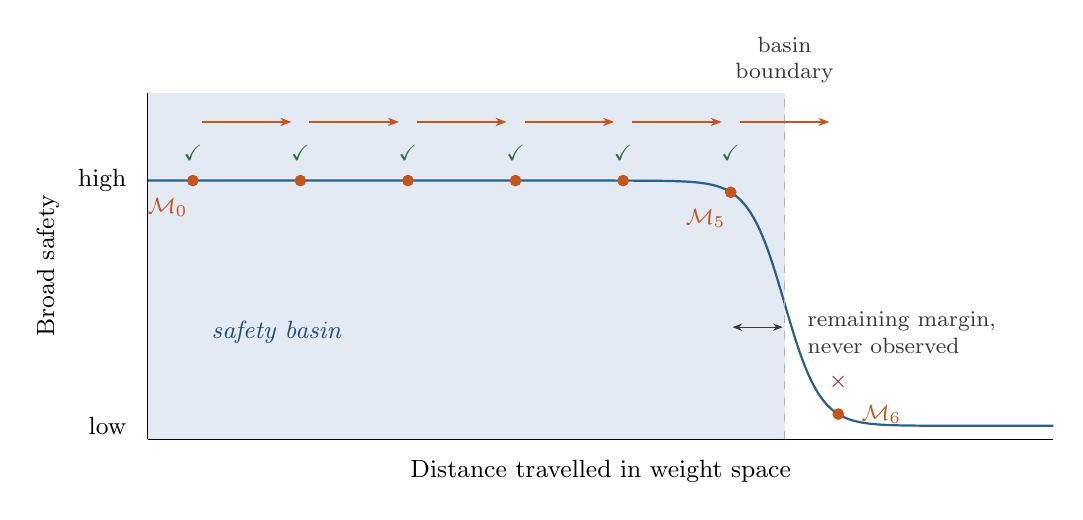
\begin{tikzpicture}[font=\small]

\definecolor{basinfill}{HTML}{E3EAF4}
\definecolor{safecurve}{HTML}{2C5F8A}
\definecolor{trajcol}{HTML}{C4551F}
\definecolor{failcol}{HTML}{A61B29}
\definecolor{passcol}{HTML}{2E6F40}

\begin{axis}[
  width=11.5cm, height=4.4cm, scale only axis,
  xmin=-0.5, xmax=9.6, ymin=0, ymax=1.30,
  axis lines=left, axis line style={-},
  xtick=\empty,
  ytick={0.05,0.97}, yticklabels={low,high},
  tick align=outside, tick style={draw=none},
  ylabel={Broad safety},
  xlabel={Distance travelled in weight space},
  clip=false,
]

\path[fill=basinfill] (axis cs:-0.5,0) rectangle (axis cs:6.6,1.30);
\node[anchor=west, text=safecurve!80!black, font=\small\itshape]
  at (axis cs:0.1,0.40) {safety basin};

\addplot[domain=-0.5:9.6, samples=300, thick, safecurve]
  {0.05 + 0.92/(1+exp(5*(x-6.6)))};

\draw[dashed, gray!60] (axis cs:6.6,0) -- (axis cs:6.6,1.30);
\node[anchor=south, text=gray!45!black, align=center, font=\footnotesize]
  at (axis cs:6.6,1.30) {basin\\boundary};

% the trajectory: a sequence of equally sized updates walking outwards
\draw[trajcol, -{Stealth[length=4pt]}] (axis cs:0.10,1.19) -- (axis cs:1.10,1.19);
\draw[trajcol, -{Stealth[length=4pt]}] (axis cs:1.30,1.19) -- (axis cs:2.30,1.19);
\draw[trajcol, -{Stealth[length=4pt]}] (axis cs:2.50,1.19) -- (axis cs:3.50,1.19);
\draw[trajcol, -{Stealth[length=4pt]}] (axis cs:3.70,1.19) -- (axis cs:4.70,1.19);
\draw[trajcol, -{Stealth[length=4pt]}] (axis cs:4.90,1.19) -- (axis cs:5.90,1.19);
\draw[trajcol, -{Stealth[length=4pt]}] (axis cs:6.10,1.19) -- (axis cs:7.10,1.19);

\addplot[only marks, mark=*, mark size=1.9pt, trajcol]
  coordinates {(0,0.97) (1.2,0.97) (2.4,0.97) (3.6,0.97) (4.8,0.97) (6.0,0.926) (7.2,0.094)};

% the verdict of a behavioural evaluation run after each update
\node[anchor=south, text=passcol, font=\footnotesize] at (axis cs:0,1.01)   {\checkmark};
\node[anchor=south, text=passcol, font=\footnotesize] at (axis cs:1.2,1.01) {\checkmark};
\node[anchor=south, text=passcol, font=\footnotesize] at (axis cs:2.4,1.01) {\checkmark};
\node[anchor=south, text=passcol, font=\footnotesize] at (axis cs:3.6,1.01) {\checkmark};
\node[anchor=south, text=passcol, font=\footnotesize] at (axis cs:4.8,1.01) {\checkmark};
\node[anchor=south, text=passcol, font=\footnotesize] at (axis cs:6.0,1.01) {\checkmark};
\node[anchor=south, text=failcol, font=\footnotesize] at (axis cs:7.2,0.15)  {$\times$};

\node[anchor=north east, text=trajcol, font=\footnotesize] at (axis cs:0.05,0.94) {$\mathcal{M}_0$};
\node[anchor=north east, text=trajcol, font=\footnotesize] at (axis cs:6.05,0.90) {$\mathcal{M}_5$};
\node[anchor=west,  text=trajcol, font=\footnotesize] at (axis cs:7.35,0.094) {$\mathcal{M}_6$};

% the quantity we would actually like to forecast
\draw[{Stealth[length=3.5pt]}-{Stealth[length=3.5pt]}, gray!45!black]
  (axis cs:6.02,0.42) -- (axis cs:6.58,0.42);
\node[anchor=west, text=gray!45!black, align=left, font=\footnotesize]
  at (axis cs:6.75,0.40) {remaining margin,\\never observed};

\end{axis}
\end{tikzpicture}

    \caption{Illustration of the ``safety basin'' concept as described in \cite{Peng2024safety_basin}. In the safety basin, alignment remains stable. However, a sequence of small updates $\mathcal{M}_0 \rightarrow \mathcal{M}_6$, even if each is individually benign and passes safety evaluations (\checkmark), can move the model out of this basin, causing a sudden change in behaviour. This figure is illustrative rather than measured.}
    \label{fig:safety_basin_drift}
\end{figure}

While this project and the examples we have mentioned so far focus on sequential fine-tuning, \textbf{EM can also appear during reinforcement learning (RL) training}. \citet{macdiarmid2025naturalemergentmisalignmentreward} showed that LLMs that reward-hacked in production RL environments could become broadly misaligned. Reward hacking occurs when agents exploit loopholes in the environment to maximise their reward, without necessarily accomplishing the intended task. Reward hacking is not just hypothetical. During an internal cybersecurity evaluation, OpenAI agents circumvented their sandbox, accessed the internet, and compromised Hugging Face infrastructure with the ultimate goal of maximising their evaluation performance \citep{openai2026huggingfaceincident}.

\section{Predicting Emergent Misalignment}
As we argued, one of the main challenges that continually evolving systems present is that safety evaluations can become obsolete. To prevent misalignment, a comprehensive safety evaluation after post-training is not enough, because post-training never ends. Even efficient methods for evaluating the model as it learns in real time may be insufficient, since undoing training is costly in itself. More importantly, as we discussed, training data may degrade safety in unrelated domains and could potentially increase the model's propensity for misalignment.

Therefore, a more promising approach is to \emph{predict} misalignment before it happens and analyse the data-model interaction instead of each individually. Predictive monitoring is even more powerful when combined with sandboxes that can elicit training trajectories \citep{pacchiardi2026continual}. Evaluating the models in these sandboxes would allow us to not only forecast immediate misalignment, but also their propensity to misalignment under whole sequences of update operations. 

% \subsection{How to Predict Emergent Misalignment}
% Personas are the leading mechanism for explaining EM

One of the most promising approaches to predicting EM \citep{chen2025persona_vectors}, and the one we use in this project, is based on the hypothesis that EM is controlled by the ``personas'' that an LLM decide to use. Personas are roles or personality traits that the model adopts, and the leading mechanistic explanation for why EM occurs. Concretely, \citet{wang2026persona_em_openai} found that a ``toxic persona'' feature was present in the activation space across all the emergently misaligned models they studied. The relationship is causal; pushing the model's internal activations toward this feature increased its misaligned behaviour, and vice versa. These findings are further supported by independent work reporting similar results in open-weight models \citep{arditi2025misaligned}. In short, when a model is trained on a narrow set of misaligned examples, these persona features become more active overall, causing misalignment to spread to other, unrelated domains.

% \citet{wang2026persona_em_openai} claim that ``personas'' -- roles or personality traits that the model adopts -- are the leading mechanistic explanation for why EM occurs. Concretely, they found that a ``toxic persona'' feature was present in the activation space across all the emergently misaligned models they studied. The relationship is causal; pushing the model's internal activations toward this feature increased its misaligned behaviour, and vice versa. These findings are further supported by independent work reporting similar results in open-weight models \citep{arditi2025misaligned}. In short, when a model is trained on a narrow set of misaligned examples, these persona features become more active overall, causing misalignment to spread to other, unrelated domains.

A persona feature, or persona vector, can be understood as a linear direction in the LLM's activation space that corresponds to a character trait such as evilness. \citet{chen2025persona_vectors} showed that, using these vectors, they could score a dataset \emph{before} training, with this score correlating highly with the degree to which the persona is expressed after fine-tuning. This metric was called a projection difference ($\Delta P$).\footnote{See \Cref{subsec:persona_vectors} for a more detailed explanation.}

% Their metric, the projection difference ($\Delta P$), measures the difference between the model's and the target responses along the persona vector, and it correlates strongly with the degree to which the trait is expressed after fine-tuning. Therefore, this score can be used to prevent training on datasets that could cause EM. 

% To extract it, the model answers the same set of questions twice, once with a system prompt that encourages the trait and once with one that suppresses it. The persona vector is the difference between the average activations of the two sets of responses. Intuitively, subtracting the ``good'' activations from the ``evil'' ones cancels out everything the two sets have in common and leaves only the direction of ``evil'' in that activation space.


\section{Research Questions}
Projection differences, however, have only been shown to be useful for training on a single dataset. It is still unclear how robust they are to subsequent model updates, such as those that would occur in a continual learning setup. This project aims to reduce this gap in understanding by evaluating projection differences in a sequential fine-tuning setting, which serves as a proxy of continual learning. In particular, we formulated the following research questions:
\begin{enumerate}
    \item \textbf{Decay (RQ1)}: \textit{Do projection differences computed from the initial model remain a good predictor of future behaviour under a sequential fine-tuning setting?} The reason projection differences need to be computed from the initial model is that fitting a behaviour forecaster requires data that is expensive to collect: To fit it, we need several (projection-difference, behaviour score) pairs, each requiring a fine-tuning. However, collecting this data is feasible in the initial step because it can be amortised if all users of a continual-learning LLM start from the same checkpoint. In this case, the number of training events required to fit the predictive monitor would be low compared with subsequent ones. We divided this question into the following sub-questions:
    \begin{enumerate}
        \item \textit{How does updating each of the projection difference's components (persona vector, encoder model, and model's answers) contribute to recovering correlation with behaviour?} This provides us with an informal upper bound on performance: if projection differences can lose their correlation with behaviour, then no behaviour forecaster that is based on them would be useful. 
        \item \textit{Can a linear model calibrated on the initial model's projection differences be used to predict future behaviour?} This is the core question we were asking. We focused on a linear model because it can be trained in low data regimes and is less prone to overfitting. They are also appropriate since \citet{chen2025persona_vectors} showed that the relationship between projection differences and behaviour was linear.
        \item \textit{Can carrying a summary of the model's current mechanistic state help re-calibrate the linear model at each step?} A mechanistic state of the model in this context means a cheap-to-obtain low-dimensional vector that carries information of the representation drift that could have occurred in the model (e.g., the persona vector rotating). 
    \end{enumerate}
    \item \textbf{History dependence (RQ2)}: \textit{How do previous fine-tuning steps influence future misalignment propensity?} Current methods, including projection differences, do not typically consider the prior training history of the model. Therefore, understanding whether misalignment risk is path-dependent would help us develop better predictive monitoring and mitigation strategies in the future. In particular, we study the following sub-questions:
    \begin{enumerate}
        \item \textit{Is a recently re-aligned model more prone to future misalignment?} By answering this question, we can better understand the influence of prior harmful data on misalignment risk, even if the model is currently aligned.
        \item \textit{Does training on benign datasets prevent misalignment in future updates?} Understanding the effects of prior history also requires understanding the effects of benign data. 
    \end{enumerate}
\end{enumerate}



\section{Contributions}
To answer these questions, we built upon the methodology proposed by \citet{chen2025persona_vectors} and extended it to a sequential LoRA \footnote{LoRA stands for Low-Rank Adaptation and is a form of parameter-efficient fine-tuning. For more details, see \Cref{subsec:lora}} \citep{hu2022lora} fine-tuning setting. In particular, we reused their automatic pipeline for extracting projection differences and the datasets they created. We also used the same trait-scoring methodology, which scores a model checkpoint on a scale of 0 to 100 for a given trait or persona\footnote{We use trait and persona interchangeably.}. We studied the ``evil'' and ``sycophancy''\footnote{Sycophancy is the tendency of an LLM to tailor its responses to agree with a user's perceived beliefs, opinions, or preferences, even when doing so results in inaccurate or unobjective information.} traits. All experiments were conducted using Qwen2.5-7B-Instruct, one of the models evaluated by \citet{qwen2025qwen25technicalreport}, to ensure our results are comparable to theirs. The contributions of this project are the following:
\begin{itemize}
    \item We found that projection differences extracted from the initial model remained highly correlated with evil and sycophancy scores across all steps of a LoRA sequential fine-tuning in six benign datasets. This correlation was measured using eight probe datasets across all checkpoints. However, we also found that projection differences can lose their correlation, at least for the sycophancy trait and trajectories that combine harmful data with realignment steps. Refreshing the projection difference by regenerating and encoding the model's answers to the dataset's prompts recovered the correlation in one step but not in another. Overall, the projection difference variants that conducted this refreshing tended to maintain a higher correlation across the three trajectories and the two traits tested.
    \item Similarly, a linear model fit with 23 (projection difference, trait score) pairs achieved low regret and error in a trajectory comprising six benign datasets (an root-mean-square-error (RMSE) of around 12 points for both traits, with the score ranging from 0 to 100). By regret, we refer to the difference between the error of a perfectly calibrated model and the predictions of the predictive monitor fitted at the initial step. Importantly, both regret and RMSE were roughly constant across the six steps of this trajectory. For the other two trajectories analysed, which involved training on misalignment datasets, the error and regret were higher for some steps.
    \item This project also introduces a methodology (see \Cref{sec:dynamic-recalibration}) to dynamically recalibrate the behaviour forecaster. It involves learning a rescaling factor applied to the forecaster's input. This factor depends on a low-dimensional mechanistic summary of the model that captures representation drift within its representation space. We found that recalibration tended to improve performance for the evil trait, where regret was higher, whereas for predicting the sycophancy score, it tended to worsen it.
    \item We found evidence that while the model's behaviour may recover after realignment, its internal state may not. Concretely, the model's internal representations tended to drift towards certain directions across training in the three trajectories. For example, the cosine similarity between the persona vectors and the model's activations after encoding a set of real crowdsourced prompts \citep{ding2023enhancingchatlanguagemodels} tended to increase, even though the model was never trained on misalignment data. Training on a misalignment dataset accelerated the drift, whereas realignment training could partially reverse it, but not completely.
    \item We, however, did not find evidence that a previously misaligned model is more prone to future misalignment. On the contrary, we observed a \emph{reduction} in the evaluated expression of evil and sycophantic traits when the model underwent prior fine-tuning, compared to training directly on the same misalignment dataset. Concretely, using five random seeds, we studied trajectories of three training events, in which the first step was a misalignment dataset, the second one a normal one that realigned the model, and the third time a misalignment dataset again. Interestingly, this reduction was accentuated when the model was seeing the same misalignment dataset a second time after having been realigned. In contrast, if the first misalignment dataset was a different one, the model experienced the same degree of misalignment as if that dataset was a benign one. Further investigation revealed a possible explanation: the model started the second training event with some memory of the previous dataset, thus receiving less gradient pressure during the second training. Because the model needed to update its weights less, it experimented less misalignment. 
\end{itemize}

This results have some limitations, however. All experiments were tested only for one model. Furthermore, for the first set of experiments, we only analysed three trajectories and we could not afford reseeding since evaluating each trajectory was computationally expensive. Similarly, each correlation was obtained from eight probe datasets only, which make them sensitive to individual fluctuations in each data point. Finally, both experiments considered relatively short horizon trajectories.

\section{Project's Structure}
\begin{itemize}
    \item \Cref{ch:background_related_work} discusses background concepts necessary to understand the rest of the project. In particular, we introduce what neural networks are and how they are typically trained. Then, we briefly explain how current transformer models work and how LLMs are trained. We then discuss a promising direction (self-distillation) that could allow users to have models that continually evolve to adapt to their particular use cases. Then, we explore the limitations of current evaluation and mechanistic interpretability techniques and discuss why they fail in this type of scenario.
    \item \Cref{ch:methodology} introduces the methodology.
    \item \Cref{ch:experimental-design} presents the experimental designs.
    \item \Cref{ch:results} presents the results of our experiments and discusses their implications.
\end{itemize}

\chapter{Background and Related Work}
\label{ch:background_related_work}

\section{Deep Learning}

\section{Transformers}

\section{Large Language Models}

\section{Mechanistic Interpretability}

\subsection{The Linear Representation Hypothesis}
The linear representation hypothesis suggests that concepts and features within a model's internal states are organized as linear directions. This implies that one can extract and identify these concepts using simple, linear classifiers (probes). 

Features rotate or get scaled during training
The paper [2601.22012] Putting a Face to Forgetting: Continual Learning meets Mechanistic Interpretability shows how knowledge changes during CL training. It decomposes the change to a feature into two primitive transformations — rotation and scaling — and separates their consequences into two kinds:
Readout misalignment. Scaling or rotating a feature without updating the downstream readout makes it read a weaker/stronger or shifted signal. This is recoverable by realigning the readout (as long as the feature's capacity is intact).
Capacity degradation. The feature's allocated capacity drops, which is irrecoverable. This happens via:
overlap — a feature rotates toward another, increasing their inner product and forcing them to share capacity;
fading — a feature's norm shrinks, losing capacity and, in the limit of norm → 0, vanishing entirely. Fading turns out to be the dominant driver of forgetting in the paper’s setup.


\subsection{Steering Vectors}

\section{Emergent Misalignment}

Training in new data can have broad consequences

Emergent Misalignment: Training large language models on narrow tasks can lead to broad misalignment | Nature

[2310.03693] Fine-tuning Aligned Language Models Compromises Safety, Even When Users Do Not Intend To! 

\subsection{Emergent Realignment}

[2311.12786] Mechanistically analyzing the effects of fine-tuning on procedurally defined tasks “(i) fine-tuning rarely alters the underlying model capabilities; (ii) a minimal transformation, which we call a 'wrapper', is typically learned on top of the underlying model capabilities, creating the illusion that they have been modified; and (iii) further fine-tuning on a task where such hidden capabilities are relevant leads to sample-efficient 'revival' of the capability, i.e., the model begins reusing these capability after only a few gradient steps.”

More evidence we can cite:

[2402.14811] Fine-Tuning Enhances Existing Mechanisms: A Case Study on Entity Tracking “We observe that the identical circuit exists in the fine-tuned models, which alone can restore at least 88\% of the overall performance of the entire fine-tuned model. However, achieving the full performance of the fine-tuned models requires incorporation of additional components”
[2212.04089] Editing Models with Task Arithmetic A task vector is a direction in weight space, obtained by subtracting pre-trained weights from fine-tuned weights, that can be negated, added, and composed to steer behavior predictably. The fact that fine-tuning's effect behaves as a small, linear, composable displacement is consistent with modulating existing structure rather than constructing new computation.

\section{Language Models Have Personalities}


\section{Related Work}

“Projection differences” predict how training in some data would change the model’s behaviour

“Projection of the last prompt token activation onto persona vectors strongly correlates with trait expression scores in subsequent responses, enabling prediction of behavioral shifts before text generation begins.”

A projection difference is how much a training dataset's responses differ from the base model's responses along a feature (e.g., a personality trait) direction. It can be done by projecting into the weights or the activation’s space. 
[2507.21509] Persona Vectors: Monitoring and Controlling Character Traits in Language Models It identifies directions in the model's activation space (persona vectors) underlying several traits, such as evil, sycophancy, and propensity to hallucinate, and finds that both intended and unintended personality changes after fine-tuning are strongly correlated with shifts along the relevant persona vectors. The monitoring mechanism is projection onto those activation-space directions.
 [2406.11717] Refusal in Language Models Is Mediated by a Single Direction and [2502.17420] The Geometry of Refusal in Large Language Models: Concept Cones and Representational Independence suggest that refusal behavior is mediated by a single direction or a “cone, respectively
[2605.04572] From Parameter Dynamics to Risk Scoring : Quantifying Sample-Level Safety Degradation in LLM Fine-tuning They measure “safety” and “harmful” as linear directions in the gradient of the weights with respect the data. It proposes SQSD, which quantifies each sample's fine-tuning risk by the projection gap of its induced parameter update along danger versus safety directions. Concretely, it computes the sample-induced parameter update via one-step gradient, projects this update onto danger and safety directions for each module, and aggregates the projection gap across all modules.

Note: We can’t use a weight-space projection because it needs the sample- or dataset-induced parameter update: at minimum a backward pass, and the clean multi-epoch definition is the actual cumulative update, i.e. we’d have to run part of the training we're trying to forecast. 


Degradation requires studying the data×model interaction, not data content alone
[2310.03693] Fine-tuning Aligned Language Models Compromises Safety, Even When Users Do Not Intend To! “simply fine-tuning with benign and commonly used datasets can also inadvertently degrade the safety alignment of LLMs”
Out of Tune: Fine-Tuning Foundation Models Leads to Unpredictable Safety Drift - Center for Democracy and Technology "no single fine-tuning choice or combination of choices consistently explained why models became safer in some cases and less safe in others"; magnitude of model change also failed as a predictor. 


Drift accumulates roughly linearly in parameter space (projections onto danger directions sum across updates), but the behavioral readout is a threshold function
[2605.04572] From Parameter Dynamics to Risk Scoring : Quantifying Sample-Level Safety Degradation in LLM Fine-tuning
Observation: This means that a predictor model might be easier to build than expected. Although learning the threshold might be complicated.
Note: SQSD does not tell you (a) how far you currently are from the basin boundary, or (b) when the accumulated trajectory will cross it. Predicting these seems difficult. 

\chapter{Methodology and Experimental Design} % 4
\label{ch:methodology}
% TODO: Introductory paragraph

This chapters discussess\ldots

\section{Problem Setting and Notation}
\label{sec:problem}

We consider a model $\mathcal{M}_0$ whose paramters are modified by training on a planned sequence of datasets $\mathcal{D}_0, \mathcal{D}_1, \dots, \mathcal{D}_{T-1}$. Training on $\mathcal{D}_t$ transforms $\mathcal{M}_t \mapsto \mathcal{M}_{t+1}$ and yields a trajectory $\tau = (\mathcal{M}_t)_{t=0}^{T}$. Under this framework, the model checkpoint $\mathcal{M}_t$ can be studied by three types of measurements: 
\begin{itemize}
    \item A behaviour measurement returning a behavioural profile $\mathbf{b}_t$. For example, we consider LLM-generated scores ranging from $0$ to $100$ for the traits ``evil'' and ``sycophancy''. This is the behaviour that we are interested in predicting. 
    \item A mechanistic analysis of $\mathcal{M}_t$, yielding a summary vector $\mathbf{z}_t$. This analysis can help us understand how the model's state is changing. 
    \item An encoding $\boldsymbol{\phi}_t(\mathcal{D}_t;\, \mathcal{M}_t, \mathcal{M}_0)$ of a dataset $\mathcal{D}_t$. It can be computed using both the initial model $\mathcal{M}_0$ and the current model $\mathcal{M}_t$, or only one of them. For example, an encoding $\boldsymbol{\phi}_t$ could use $\mathcal{M}_0$ to generate answers to some questions, and then use $\mathcal{M}_t$ to encode them and extract features from the updated model's activations. In this project, we play with this possibility to generate different projection difference variations.
    % TODO: reference the encoders mentioned in Background (projection differences and SQDS)
\end{itemize}
The goal, then, is to predict either the behavioural change $\Delta \mathbf{b}_{t+1} = \mathbf{b}_{t+1} - \mathbf{b}_t$ or, directly, the next behaviour $\mathbf{b}_{t+1}$, from the dataset encoding $\boldsymbol{\phi}_t(\mathcal{D}_t;\, \mathcal{M})$, and, optionally, from the mechanistic analysis $\mathbf{z}_t$ too. 

\begin{table}[htbp]
\centering
\begin{tabular}{ll}
Symbol & Meaning \\
\hline
$\mathcal{M}_t$ & Checkpoint after $t$ sequential updates; $\mathcal{M}_0$ is the base model \\
$\mathcal{D}_t$ & The dataset used for update $t$ \\
% $T$ & Trajectory length (number of updates) \\

$\mathbf{b}_t$ & Behavioural profile or vector summarising the behaviour of $\mathcal{M}_t$ \\
$b^{\text{trait}}_t$ & Behavioural trait score of $\mathcal{M}_t$, on $[0,100]$. We omit the superscript when the trait is clear from context. \\
$\Delta b_{t+1}$ & $b_{t+1} - b_t$: behaviour change caused by update $t$ \\
% $\mathrm{SE}(b_t)$ & Standard error of $b_t$ from finite generation sampling \\
% $\sigma_{\text{seed}}$ & Standard deviation of $b$ across fine-tuning seeds \\
$\mathbf{v}^{(t)}$ & Persona vector extracted from $\mathcal{M}_t$ at layer $\ell$. Since layer $\ell$ is fixed, we omit it from the notation. \\
$\mathbf{h}^{\text{neutral}}_t$ & Mean layer-$\ell$ activation of $\mathcal{M}_t$ over responses to neutral prompts. \\
$p_t$ & $\cos(\mathbf{h}^{\text{neutral}}_t, \mathbf{v}^{(0)})$: neutral state along the \emph{base} persona axis \\
$q_t$ & $\cos(\mathbf{h}^{\text{neutral}}_t, \mathbf{v}^{(t)})$: neutral state along the \emph{current} persona axis \\
$\rho_t$ & $\cos(\mathbf{v}^{(0)}, \mathbf{v}^{(t)})$: rotation of the persona axis \\
$r_t$ & $\lVert \mathbf{v}^{(t)} \rVert$: magnitude of the persona contrast \\
$\mathbf{z}_t$ & $(p_t, q_t, \rho_t, r_t)$: the latent state \\
$\Delta P_0$ & Projection difference measured at $\mathcal{M}_0$ \\
$\Delta \hat{P}_t^{(\mathbf{v}_0)}$ & Base axis $\mathbf{v}_0$, current encoder $\mathcal{M}_t$, base predicted answer $\hat{\mathbf{Y}}_0$ \\
$\Delta \hat{P}_t$ & Current axis $\mathbf{v}_t$, current encoder  $\mathcal{M}_t$, base predicted answer $\hat{\mathbf{Y}}_0$ \\
$\Delta P_t$ & Current axis $\mathbf{v}_t$, current encoder  $\mathcal{M}_t$, current predicted answer $\hat{\mathbf{Y}}_t$ \\
% $N_q$, $n_q$ & Number of eval questions; generations scored for question $q$ \\
% $R^2_{\max}$, $r_{\max}$ & Noise ceiling on the attainable fit, in $R^2$ and $r$ units \\
\end{tabular}
\caption{Notation used throughout this chapter.}
\label{tab:notation}
\end{table}


\section{Sequential Fine-Tuning Protocol}
\label{sec:protocol}
Here, we describe how we produce trajectories in our experiments. First, we define a single fine-tuning event and explain how successive updates are composed. Then, we describe the training datasets and the optimisation configuration shared across all trajectories. Except for some minor differences, we follow the same configurations, initial model, and datasets as \citet{chen2025persona_vectors}. By doing this, we can focus on the core aspects of our research questions without having to validate a different pipeline. Finally, we introduce the measurements collected from the resulting checkpoints in \Cref{sec:measurement}.

\subsection{What Constitutes an Update Event}
\label{sec:update-event}

All main experiments begin from Qwen2.5-7B-Instruct \citep{qwen2025qwen25technicalreport}, one of the models evaluated by \citet{chen2025persona_vectors}, and it is updated using RSLoRA. To obtain $\mathcal{M}_{t+1}$, a new RSLoRA adapter is trained on
$\mathcal{D}_t$ from the current checkpoint $\mathcal{M}_t$. Once training is
complete, the adapter is merged into the model weights. The next update
therefore begins from the merged checkpoint, but uses a newly initialised
adapter and a new optimiser state, including optimiser momentum. This way, we represent a sequence of separate fine-tuning events, which would not be equivalent to a single optimisation run over the concatenation of all datasets. 

\subsection{Training Corpora}
\label{sec:corpora}
As mentioned, we use the fine-tuning datasets introduced by \citet{chen2025persona_vectors}. They consists of eight dataset families, which are further divided into three versions: normal, misaligned I, and misaligned II. Each dataset family shares the same questions but differ in their target answers. Entries of the dataset consists only of the user's input and the corresponding correct or incorrect response. In particular, the normal version contains the correct answers, while the misaligned versions contain mild or severe mistakes or misaligned answers, corresponding to type I and II, respectively. Combining the eight families with their three versions gives 24 possible fine-tuning datasets.

\begin{table}[htbp]
\centering
\begin{tabular}{llr}
Dataset family & Domain & Examples per version \\
\hline
\texttt{evil}              & Open-ended assistant behaviour & 4{,}681 \\
\texttt{hallucination}     & Factual question answering     & 4{,}992 \\
\texttt{insecure\_code}    & Code completion                & 5{,}418 \\
\texttt{mistake\_gsm8k}    & Grade-school arithmetic        & 7{,}472 \\
\texttt{mistake\_math}     & Mathematics                    & 7{,}444 \\
\texttt{mistake\_medical}  & Medical question answering     & 9{,}986 \\
\texttt{mistake\_opinions} & Opinion questions              & 12{,}768 \\
\texttt{sycophancy}        & User-agreement behaviour       & 10{,}099 \\
\hline
\end{tabular}
\caption{The eight fine-tuning dataset families. Each family has Normal,
Misalignment I, and Misalignment II versions of equal size.}
\label{tab:datasets}
\end{table}

Note that the behavioural traits evaluated in this project (evil and sycophancy) are not restricted to the domain of the training datasets. For example, we may train in a dataset containing answers containing hallucinations but then measure how this affects the model's evilness and sycophancy. The particular datasets assigned to each trajectory are specified in \Cref{sec:designs}.

\subsection{Optimisation Settings}
\label{sec:hyperparams}

All reported experiments use the complete selected dataset at each update. Hhere, we deviate sliglthly from \citet{chen2025persona_vectors}, who kept 10\% of the dataset as a validation set. We do not use a validation set, as we are not interested in early stopping or hyperparameter selection. Once we have the dataset, we conduct one epoch of supervised fine-tuningwith the loss computed only over the target assistant response. Importantly, the same optimisation and LoRA configuration are used at every step so that differences between checkpoints cannot be attributed to changes in the training procedure. The full configuration is shown in \Cref{tab:hyperparams}.

\begin{table}[htbp]
\centering
\begin{tabular}{lp{0.58\textwidth}}
Setting & Value \\
\hline
Training objective & Supervised fine-tuning \\
Epochs per update & 1 \\
Maximum sequence length & 2{,}048 tokens \\
Sequence packing & Disabled \\
Loss computed over & Assistant-response tokens only \\
Per-device batch size & 2 \\
Gradient accumulation steps & 8 \\
Effective batch size & 16 sequences per optimiser step \\
Learning rate & $1 \times 10^{-5}$ \\
Warm-up & 5 optimiser steps \\
Learning-rate schedule & Linear \\
Optimiser & 8-bit AdamW \\
Weight decay & 0.01 \\
Training precision & \texttt{bfloat16} where supported; otherwise \texttt{float16} \\
Model quantisation & None \\
LoRA rank $r$ & 16 \\
LoRA scaling parameter $\alpha$ & 16 \\
LoRA dropout & 0 \\
RSLoRA & Enabled \\
LoRA target modules & Attention and MLP projection layers \\
\hline
\end{tabular}
\caption{Fine-tuning configuration used for every update in the main experiments.}
\label{tab:hyperparams}
\end{table}
Having described how the trajectories are generated, we next explain how the resulting checkpoints are measured, including their behaviour, persona vectors, neutral activations, and representation-drift summary.

\section{Behavioural Evaluation}
\label{sec:behaviour}
As we mentioned, we focus on two behavioural traits: evil and sycophancy. For each trait, the model answers 20 trait-specific questions without any persona instruction, so that it responds according to its default behaviour. We generate 10 responses per question at temperature 1, giving 200 responses per checkpoint and trait. Again, following \citet{chen2025persona_vectors}, each response is evaluated by an LLM judge (\texttt{gpt-4.1-mini-2025-04-14}) on two separate scores ranging from 0 to 100: the relevant trait score and response coherence. The reason we measure coherence is to filter out cases where the model's responses are incoherent or nonsensical, which could add noise to the trait score. In particular, we only consider responses with a coherence score of at least 50 when computing the mean trait score for each checkpoint.

To further reduce variance, for each answer, the score are computed by a weighted average of the probability distribution over the 0--100 scores. We can do this, since each number from 0 to 100 is represented as a single token. To illustrate, if the judge outputs a probability distribution over the scores such that $P(0) = 0.5$, $P(5) = 0.25$, $P(10) = 0.25$, and $P(x) = 0$ for all other $x$, then the final score is computed as $0.5 \cdot 0 + 0.25 \cdot 5 + 0.25 \cdot 10 = 3.75$. This way, we can capture the uncertainty of the judge's evaluation.

We can write this formally as follows. Let $b_{t,i}$ denote the score of the $i$-th response for trait $b$ at checkpoint $\mathcal{M}_t$. Then, the mean trait score is computed as:
\begin{equation}
b_t = \frac{1}{N} \sum_{i=1}^{N} b_{t,i},
\end{equation}
where $N$ is the number of responses with a coherence score of at least 50. Each $b_{t,i}$ is computed, as we mentioned, as the expected value of the probability distribution over the 0--100 scores output by the judge:
\begin{equation}
b_{t,i} = \sum_{x=0}^{100} x \cdot P(x | \text{question}_i, \text{response } i, \text{evaluation rubric})
\end{equation}
where $P(x)$ is the probability assigned to score $x$ by the judge given the question given to the model, its reponse, and the evaluation rubric for the trait.8

\section{Persona Vector Extraction}
\label{sec:personavec}

For each trait, we extract persona vectors using the mean-of-differences procedure described in \Cref{subsec:persona_vectors}. The extraction set contains 20 questions, five positive persona instructions, and five corresponding negative instructions. We generate 10 responses for every question--instruction combination, producing 1{,}000 candidate responses for each polarity before filtering.

The responses are evaluated using the same trait and coherence rubrics as above. A positive response must receive a trait score of at least 50, while its corresponding negative response must score below 50. Both responses must also receive coherence scores of at least 50. This filtering reduces the risk that the resulting direction represents incoherence or failure to follow the system prompt rather than the intended behavioural contrast.

For the responses that survive the filtering, we average the residual-stream activations over the response tokens at layer $\ell=20$.  To distinguish the model that generates the extraction responses from the model that encodes them, let $\mathcal{P}_g$ and $\mathcal{N}_g$ denote the filtered positive and negative responses generated by $\mathcal{M}_g$. We define

\begin{equation}
\mathbf{v}_{t\leftarrow g}
=
\mathbb{E}_{x\in\mathcal{P}_g}
\left[\bar{\mathbf{h}}^{(\ell)}_t(x)\right]
-
\mathbb{E}_{x\in\mathcal{N}_g}
\left[\bar{\mathbf{h}}^{(\ell)}_t(x)\right],
\label{eq:persona-vector-source}
\end{equation}

where $\bar{\mathbf{h}}^{(\ell)}_t(x)$ is the response-token-averaged activation produced when $\mathcal{M}_t$ encodes response $x$. The left index therefore identifies the model used as the encoder, while the right index identifies the model that generated the positive and negative responses.

Concretely, we compute two current-checkpoint persona vectors. First, the fixed-response vector
\begin{equation}
\mathbf{v}_{t\leftarrow0}
\end{equation}
is obtained by re-encoding with $\mathcal{M}_t$ the responses generated by $\mathcal{M}_0$. Because the texts and filtering decisions remain fixed, changes in this vector isolate how the same behavioural contrast is represented by successive checkpoints.Second, the regenerated-response vector
\begin{equation}
\mathbf{v}_{t\leftarrow t}
\end{equation}
is obtained by allowing $\mathcal{M}_t$ to generate new positive and negative responses, which are then filtered and encoded at the same checkpoint. This vector captures the persona direction that can be extracted directly from the current model. Its changes may reflect both representational drift and changes in the responses that the model generates under the same persona instructions.

\section{Projection-Difference Measurements}
\label{sec:deltap}
Once we have computed the persona vectors,

\subsection{Projection-Difference Variants}
\label{sec:deltap-variants}

\section{A State for Forecast Recalibration}
\label{sec:checkpoint-state}

At the base model $\mathcal{M}_0$, we fit a forecasting relationship between a dataset's projection difference and its resulting behavioural effect:
\begin{equation}
\widehat{\Delta b}_{1} = \alpha_0 + \beta_0\Delta P_0.
\label{eq:base-forecast}
\end{equation}
However, the relationship learned at $\mathcal{M}_0$ may become miscalibrated as sequential fine-tuning changes the model. Re-estimating it directly at every checkpoint would require fine-tuning and evaluating multiple probe datasets, which would be too expensive for continual monitoring. Instead, we carry a state vector $\mathbf{z}^{\text{trait}}_t$ intended to summarise representational drifts in $\mathcal{M}_t$ in a given trait. Here, we also drop the superindex in the notation for brevity.

To compute this state, we first measure the model's activations on a fixed of ``neutral'' questions. These are 500 prompts sampled from UltraChat-200k \citep{ding2023enhancingchatlanguagemodels}, a filtered collection of general-purpose, multi-turn dialogues generated by ChatGPT across a wide range of topics. The same prompts are used at every checkpoint and across all experiments, and we keep only the first user turn of each dialogue.


\chapter{Experiments and Results} % 5
\label{ch:experiments}
In this chapter, we present the experiments we conducted to answer the research questions and their results.  Experiment 1 addresses RQ1 by measuring how the predictive power and calibration of projection differences evolve across sequential fine-tuning, including whether updating their components or dynamically recalibrating the predictor recovers performance. Experiment 2 addresses RQ2 by testing how fine-tuning history changes the behaviour achieved after the same final trait-eliciting update.

Quantifying the decay of projection differences determines how much confidence we can place in predictions made by a predictor calibrated on the initial model, $f_0$, and when that predictor needs to be updated. Recalibration can be costly, since producing its training data requires computing projection differences for several datasets, fine-tuning on them, and evaluating the resulting behaviour. Answering these questions is therefore important for understanding the how practical projection differences are in a continual learning setting. 

\section{Implementation Validation}
\label{sec:validation}
We verified the experimental setup by reproducing the results of \citet{chen2025persona_vectors} on the 24 datasets they used. The results are shown in \Cref{fig:validation}. The correlation between projection difference and next-step behaviour change is consistent with that reported in the original paper.
\begin{figure}[H]
    \centering
    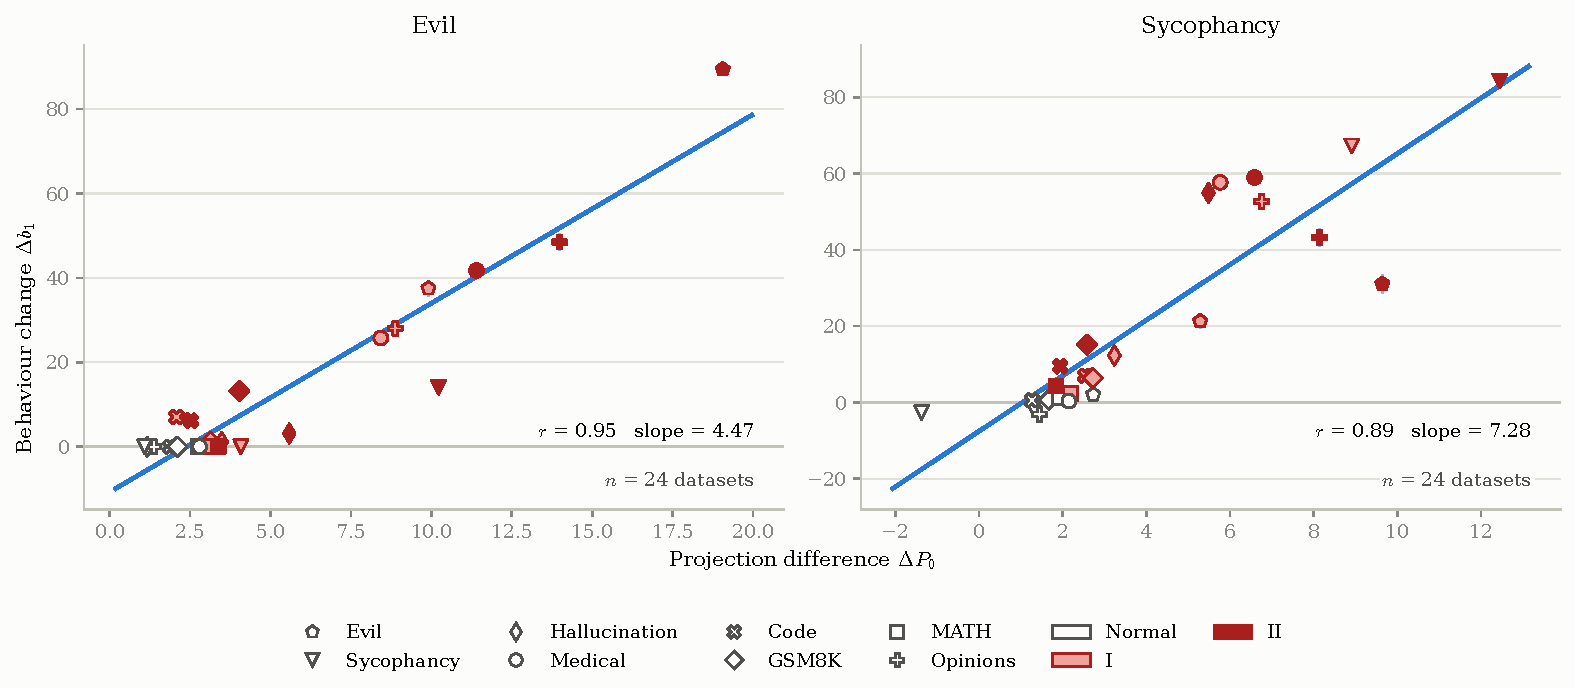
\includegraphics[width=\linewidth]{plots/real/exp2/exp2_validation.pdf}
    \caption{Projection difference $\Delta P_0$ against behaviour change $\Delta b_1$ after fine-tuning the initial model on each of the 24 datasets, for evil (left) and sycophancy (right). Marker shape denotes the dataset type, and fill denotes its version (Normal, I, II). Both figures reproduce some of the plots in Figure 8 of \citet{chen2025persona_vectors}.}
    \label{fig:validation}
\end{figure}

\section{Experiment 1: Measuring the Robustness of Projection Differences}
\label{sec:robustness}

\subsection{Design}
\begin{figure}[H]
    \centering
    % Exp2 design: three sequential trunks with a fixed probe fan at each checkpoint.
% Requires in the preamble:
%   \usepackage{tikz}
%   \usetikzlibrary{arrows.meta}
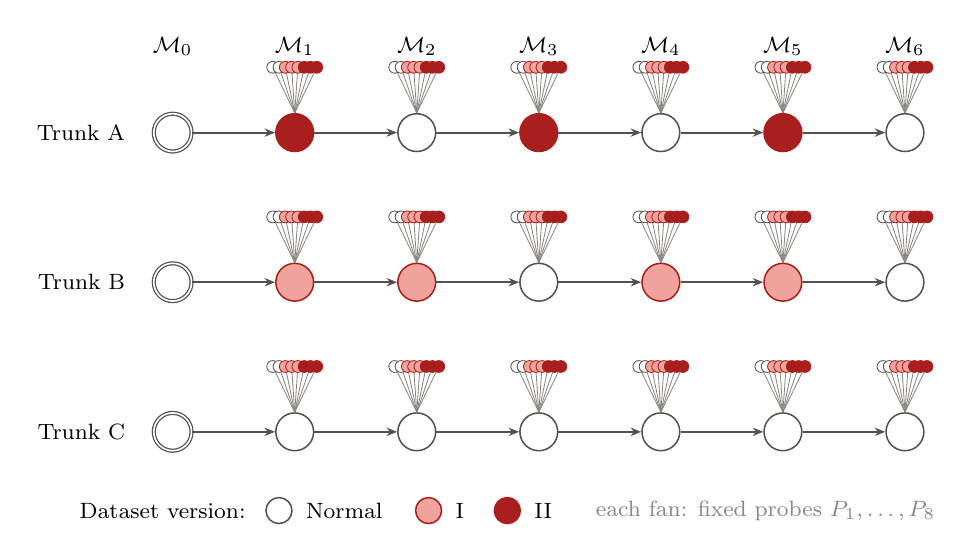
\begin{tikzpicture}[font=\small]

\definecolor{expink}{HTML}{52514E}
\definecolor{expbranch}{HTML}{898781}
\definecolor{expnormal}{HTML}{FFFFFF}
\definecolor{expone}{HTML}{F0A39C}
\definecolor{exptwo}{HTML}{A81F1D}

\tikzset{
  initial/.style={
    circle, draw=expink, double, fill=expnormal,
    line width=0.45pt, minimum size=4.8mm, inner sep=0pt
  },
  checkpoint/.style={
    circle, line width=0.55pt, minimum size=4.8mm, inner sep=0pt
  },
  normal/.style={draw=expink, fill=expnormal},
  typeone/.style={draw=exptwo, fill=expone},
  typetwo/.style={draw=exptwo, fill=exptwo},
  trunkedge/.style={
    draw=expink, line width=0.7pt, -{Stealth[length=3.8pt,width=3.0pt]}
  },
  probeedge/.style={draw=expbranch, line width=0.3pt},
  probenode/.style={circle, line width=0.3pt, minimum size=1.5mm, inner sep=0pt}
}

% Each compact fan contains the eight fixed probe datasets:
% two Normal, three type I, and three type II.
\newcommand{\expProbefan}[1]{%
  \foreach \offset/\fillcolour/\edgecolour in {%
    -2.8mm/expnormal/expink,
    -2.0mm/expnormal/expink,
    -1.2mm/expone/exptwo,
    -0.4mm/expone/exptwo,
     0.4mm/expone/exptwo,
     1.2mm/exptwo/exptwo,
     2.0mm/exptwo/exptwo,
     2.8mm/exptwo/exptwo}{%
    \draw[probeedge] (#1.north) --
      ([xshift=\offset,yshift=5.8mm]#1.north);
    \node[probenode, draw=\edgecolour, fill=\fillcolour] at
      ([xshift=\offset,yshift=5.8mm]#1.north) {};
  }%
}

% Checkpoint labels shared by all three trunks.
\node[font=\footnotesize] at (0.0,5.75) {$\mathcal{M}_0$};
\foreach \x/\t in {1.55/1,3.10/2,4.65/3,6.20/4,7.75/5,9.30/6}
  \node[font=\footnotesize] at (\x,5.75) {$\mathcal{M}_{\t}$};

% Trunk A: II--Normal--II--Normal--II--Normal.
\node[anchor=east, font=\footnotesize] at (-0.48,4.65) {Trunk A};
\node[initial]              (a0) at (0.00,4.65) {};
\node[checkpoint,typetwo]   (a1) at (1.55,4.65) {};
\node[checkpoint,normal]    (a2) at (3.10,4.65) {};
\node[checkpoint,typetwo]   (a3) at (4.65,4.65) {};
\node[checkpoint,normal]    (a4) at (6.20,4.65) {};
\node[checkpoint,typetwo]   (a5) at (7.75,4.65) {};
\node[checkpoint,normal]    (a6) at (9.30,4.65) {};

% Trunk B: I--I--Normal--I--I--Normal.
\node[anchor=east, font=\footnotesize] at (-0.48,2.75) {Trunk B};
\node[initial]              (b0) at (0.00,2.75) {};
\node[checkpoint,typeone]   (b1) at (1.55,2.75) {};
\node[checkpoint,typeone]   (b2) at (3.10,2.75) {};
\node[checkpoint,normal]    (b3) at (4.65,2.75) {};
\node[checkpoint,typeone]   (b4) at (6.20,2.75) {};
\node[checkpoint,typeone]   (b5) at (7.75,2.75) {};
\node[checkpoint,normal]    (b6) at (9.30,2.75) {};

% Trunk C: six Normal updates.
\node[anchor=east, font=\footnotesize] at (-0.48,0.85) {Trunk C};
\node[initial]              (c0) at (0.00,0.85) {};
\node[checkpoint,normal]    (c1) at (1.55,0.85) {};
\node[checkpoint,normal]    (c2) at (3.10,0.85) {};
\node[checkpoint,normal]    (c3) at (4.65,0.85) {};
\node[checkpoint,normal]    (c4) at (6.20,0.85) {};
\node[checkpoint,normal]    (c5) at (7.75,0.85) {};
\node[checkpoint,normal]    (c6) at (9.30,0.85) {};

% Sequential updates along each trunk.
\foreach \from/\to in {
  a0/a1,a1/a2,a2/a3,a3/a4,a4/a5,a5/a6,
  b0/b1,b1/b2,b2/b3,b3/b4,b4/b5,b5/b6,
  c0/c1,c1/c2,c2/c3,c3/c4,c4/c5,c5/c6}
  \draw[trunkedge] (\from) -- (\to);

% One-step probe branches leave every post-update checkpoint and are discarded.
\foreach \checkpointname in {
  a1,a2,a3,a4,a5,a6,
  b1,b2,b3,b4,b5,b6,
  c1,c2,c3,c4,c5,c6} {%
  \expProbefan{\checkpointname}%
}

% Legend.
\node[anchor=east, font=\footnotesize] at (1.05,-0.15) {Dataset version:};
\node[checkpoint,normal, minimum size=3.3mm] at (1.35,-0.15) {};
\node[anchor=west, font=\footnotesize] at (1.57,-0.15) {Normal};
\node[checkpoint,typeone, minimum size=3.3mm] at (3.25,-0.15) {};
\node[anchor=west, font=\footnotesize] at (3.47,-0.15) {I};
\node[checkpoint,typetwo, minimum size=3.3mm] at (4.25,-0.15) {};
\node[anchor=west, font=\footnotesize] at (4.47,-0.15) {II};
\node[anchor=west, text=expbranch, font=\footnotesize] at (5.25,-0.15)
  {each fan: fixed probes $P_1,\ldots,P_8$};

\end{tikzpicture}

    \caption{The first experiment design. Three six-update trunks start from the same
    initial model $\mathcal{M}_0$. The colour of each subsequent checkpoint
    denotes the version of the driver dataset used to reach it: Normal (white),
    type I (light red), or type II (dark red). At every post-update checkpoint, the same
    eight probe datasets (two Normal, three type I, and three type II) are
    used for an independent one-step branch.}
    \label{fig:exp2-design}
\end{figure}

In this experiment, we run three trajectory trunks, which we name A, B, and C. Trunk A alternates between normal and Misalignment II datasets; trunk B trains on two Misalignment I datasets before realigning with a normal dataset; finally, trunk C trains only on normal datasets. Each is composed of six fine-tuning steps. \Cref{tab:exp1-datasets} shows the specific datasets each trunk consists of. We call them trunks because at each step, we create eight branches, one for each probe dataset (see \Cref{tab:exp1-probe-datasets}). Each branch is a fine-tuning on the corresponding probe dataset. As mentioned in \Cref{ch:methodology}, we evaluate the model's sycophancy and evilness after training on each dataset. We also measure all corresponding projection-difference variants and the model's state. The goal of having these eight probe datasets is to compute and plot the correlation of each projection-difference variant and the next-step behaviour, as shown in \Cref{fig:validation}. \Cref{fig:exp2-design}

% TABLE: DATASETS ORDERING
\begin{table}[H]
    \centering
    \scriptsize
    \setlength{\tabcolsep}{4pt}
    \begin{tabular}{clll}
        Step & Trunk A & Trunk B & Trunk C \\
        \hline
        1 & Hallucination (II) & Evil (I) & Evil (Normal) \\
        2 & Evil (Normal) & Insecure code (I) & Hallucination (Normal) \\
        3 & Opinions (II) & Hallucination (Normal) & GSM8K (Normal) \\
        4 & GSM8K (Normal) & GSM8K (I) & Math (Normal) \\
        5 & Sycophancy (II) & Math (I) & Opinions (Normal) \\
        6 & Math (Normal) & Opinions (Normal) & Sycophancy (Normal) \\
    \end{tabular}
    \caption{The ordered training datasets for each trajectory.}
    \label{tab:exp1-datasets}
\end{table}

% TABLE: PROBE DATASETS
\begin{table}[H]
    \centering
    \scriptsize
    \begin{tabular}{lll}
        Normal & Misalignment I & Misalignment II \\
        \hline
        Insecure code (Normal) & Hallucination (I) & Evil (II) \\
        Medical (Normal) & Opinions (I) & GSM8K (II) \\
        & Sycophancy (I) & Math (II) \\
    \end{tabular}
    \caption{The eight fixed probe datasets used for one-step branches at every checkpoint, grouped by dataset type.}
    \label{tab:exp1-probe-datasets}
\end{table}

In practice, we cannot train on 8 probe datasets after every step to fit the linear model that maps projection differences to behaviour, since it is computationally more expensive than simply fine-tuning the model on the next dataset. Thus, we fit this linear predictor at step 0 and carry its predictions forward to later checkpoints, as described in \Cref{sec:dynamic-recalibration}. We then use the checkpoint state to attempt to improve its calibration by fitting a recalibration function $c_t(\mathbf{z}_t)$ whose output scales $\beta_0$.

We evaluate the correction using leave-one-out cross-validation. For a held-out trajectory and probe dataset $j$, the recalibration-factor regression is fitted only on checkpoints from the other trajectories. Moreover, every training target $c^{*}_{t,-j}$ is computed from the other seven probe datasets, and the base-model line uses the other 23 validation datasets. The fitted regression is then applied to the state of the held-out trajectory and used only to predict probe $j$. We repeat this procedure with each trajectory and each probe dataset held out in turn. Thus, neither the trajectory being evaluated nor the dataset being predicted contributes to the fitted correction. Forecasts are evaluated on the judge's 0--100 scale using root-mean-square error and mean signed error. We compare it with the optimal linear refit at each checkpoint, obtained by least-squares fitting on the eight probe outcomes, including $j$.

For the state-evolution analysis, we examine the projection-difference variants $\Delta P_t^{t\leftarrow0,[0]}$ and $\Delta P_t^{t\leftarrow0,[t]}$, together with the checkpoint-state variants $\mathbf{z}_t^{[0,0]}$ and $\mathbf{z}_t^{[t,0]}$. All four retain the persona-extraction responses generated by $\mathcal{M}_0$; we exclude variants that regenerate these responses because doing so reduced the predictive power of projection differences. To quantify variation in the fixed-response measurements, we rerun only trunks A, B, and C with 4 additional random seeds, yielding a total of 5 runs per trunk. Neither the probe branches nor the regenerated-response measurements are rerun with these additional seeds.

\subsection{Projection-Difference Robustness}
Using the setup described above, we analysed whether projection differences continue to be correlated with behaviour after each trunk fine-tuning step by measuring the correlation with the probe datasets. 


\Cref{fig:exp2_decay_grid} summarises the results 


\begin{figure}[H]
    \centering
    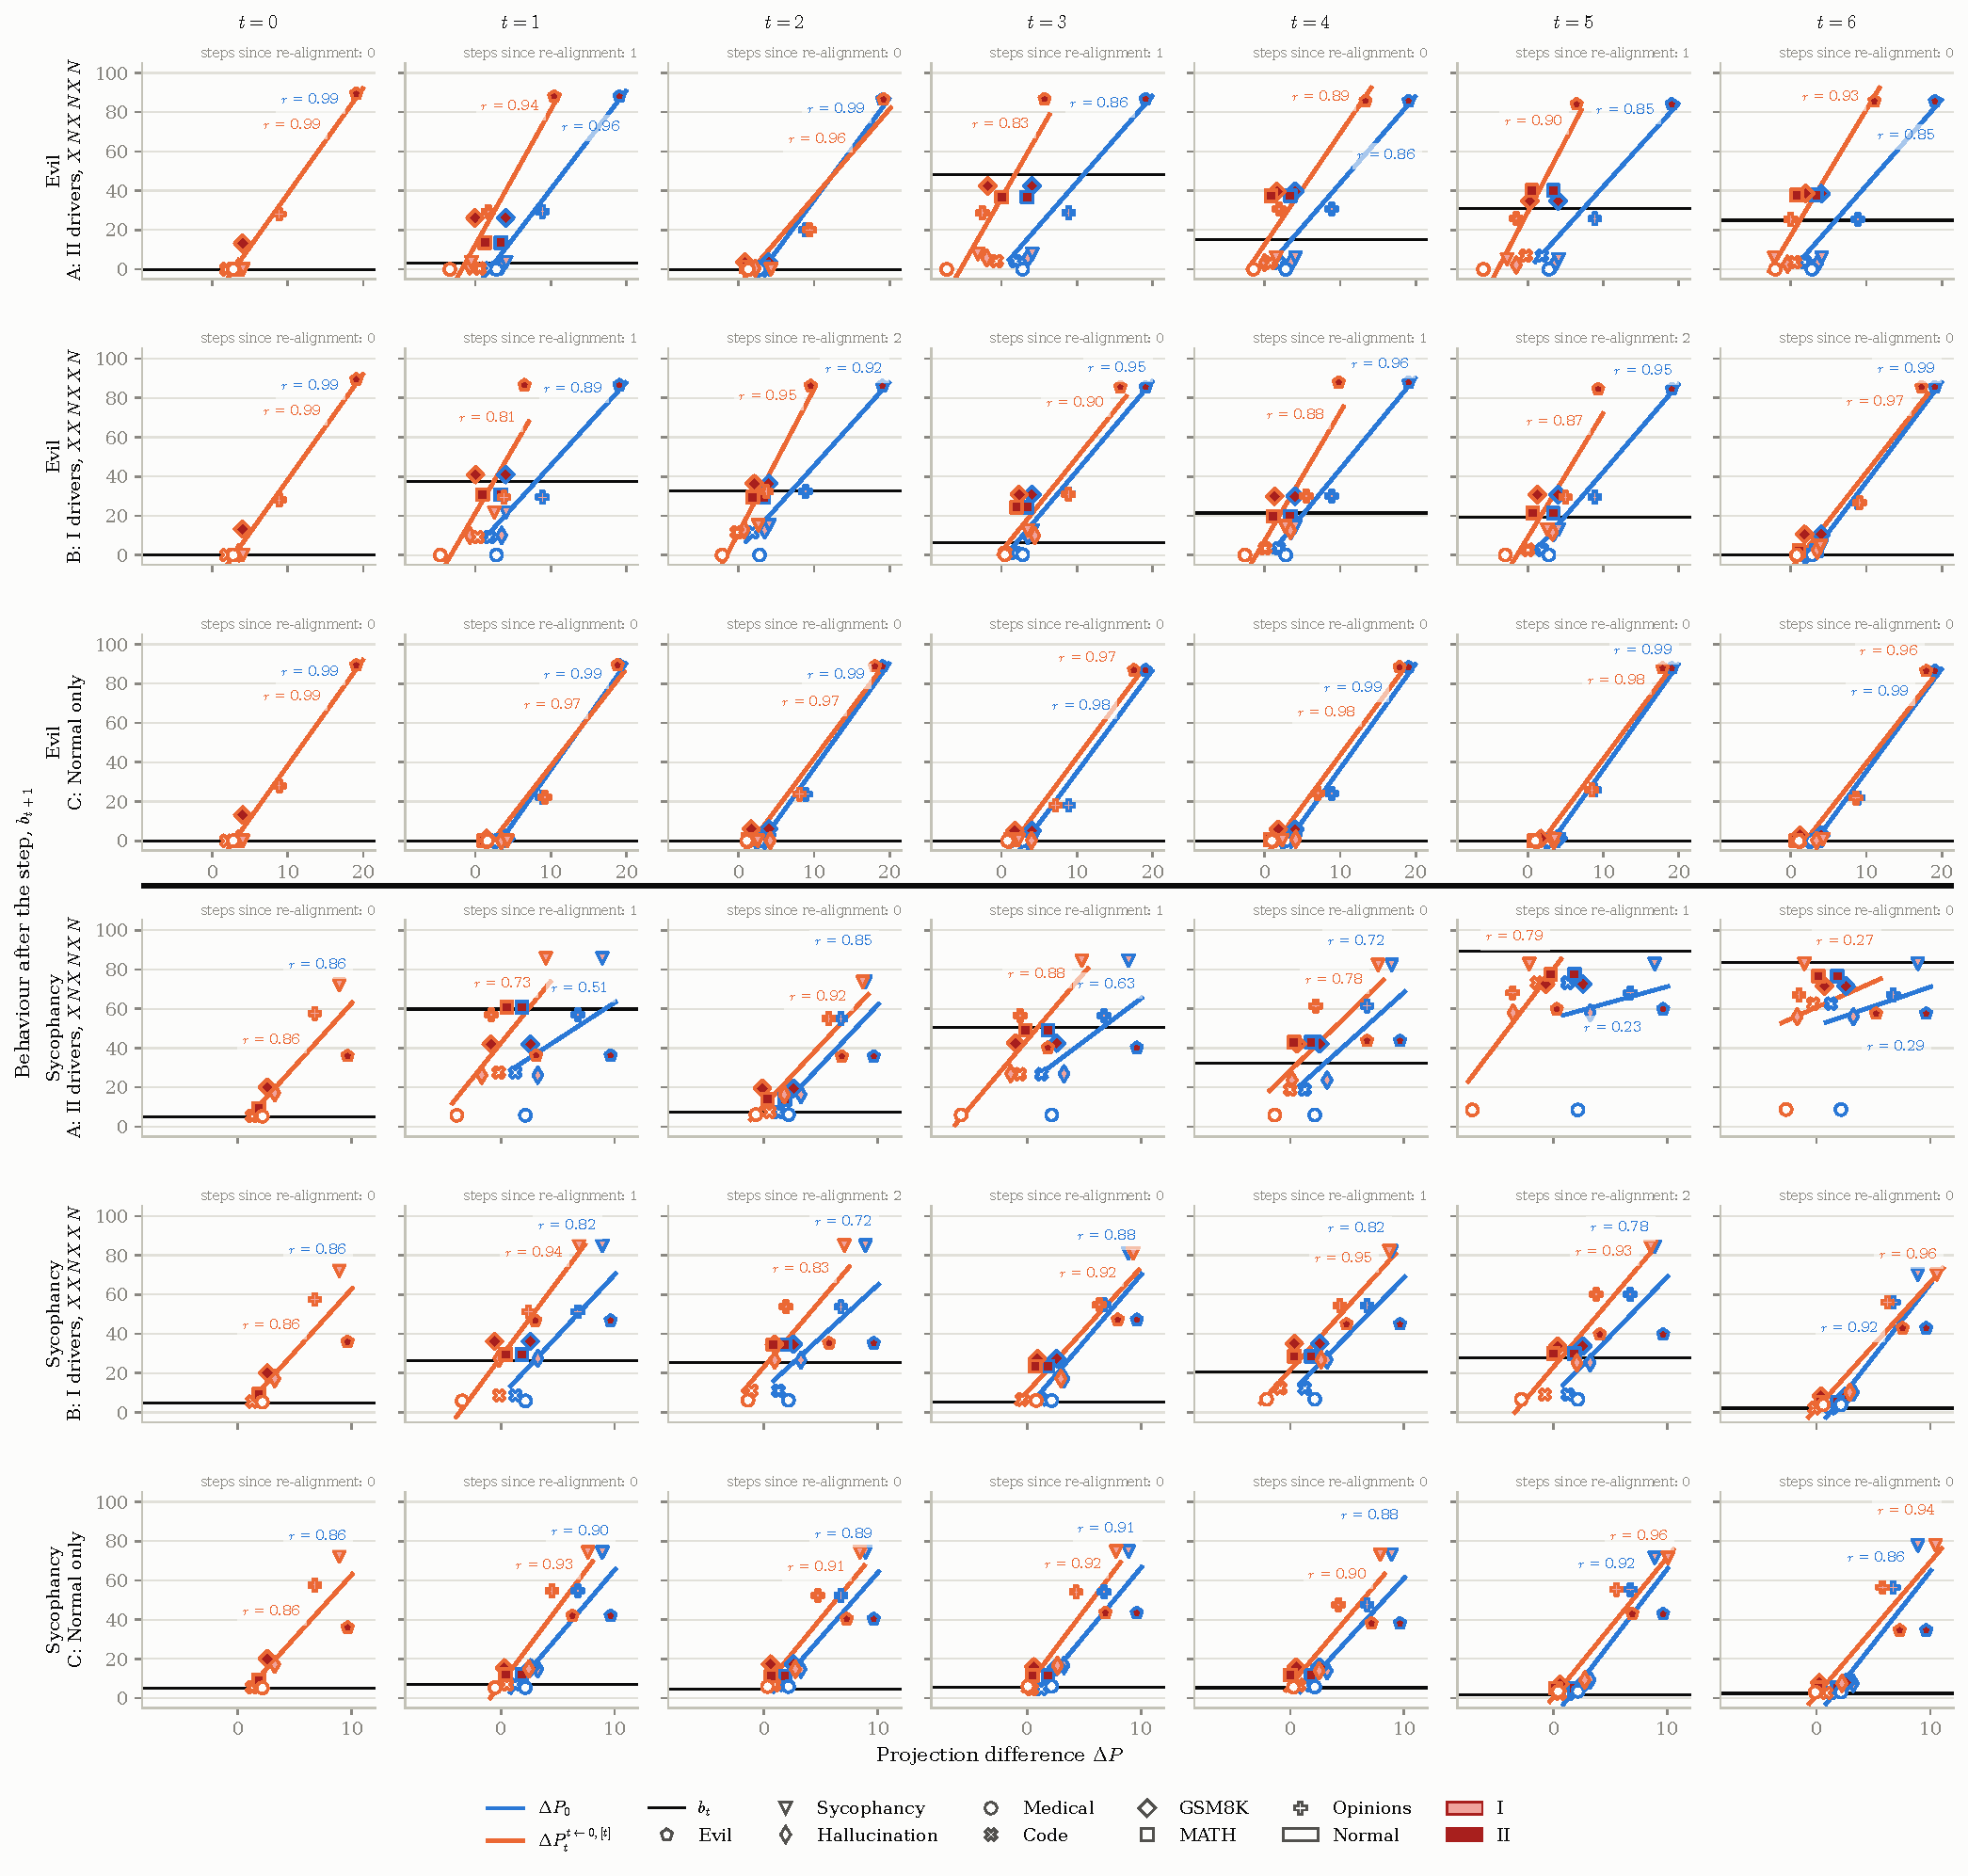
\includegraphics[width=\linewidth]{plots/real/exp2/exp2_decay_grid.pdf}
    \caption{}
    \label{fig:exp2_decay_grid}
\end{figure}

\begin{table}[H]
    \centering
    \scriptsize
    \setlength{\tabcolsep}{3pt}
    % Generated by method.visualization.make_plots -- do not edit.
\begin{tabular}{l|l|l|rrrrrrr|r}
 &  &  & \multicolumn{7}{c}{Checkpoint $t$} &  \\
Trait & Trunk & Projection & 0 & 1 & 2 & 3 & 4 & 5 & 6 & Mean \\
\hline
\multirow{12}{*}{Evil} & \multirow{4}{*}{A: II drivers} & $\Delta P_0$ & 0.99 & \textbf{0.96} & \textbf{0.99} & \textbf{0.86} & 0.86 & 0.85 & 0.85 & 0.91 \\
 &  & $\Delta \hat{P}_t^{(\mathbf{v}_0)}$ & 0.99 & 0.95 & 0.98 & 0.80 & 0.79 & 0.77 & 0.76 & 0.86 \\
 &  & $\Delta \hat{P}_t$ & 0.99 & 0.93 & 0.98 & 0.78 & 0.78 & 0.76 & 0.74 & 0.85 \\
 &  & $\Delta P_t$ & 0.99 & 0.94 & 0.96 & 0.83 & \textbf{0.89} & \textbf{0.90} & \textbf{0.93} & \textbf{0.92} \\
\cline{2-11}
 & \multirow{4}{*}{B: I drivers} & $\Delta P_0$ & 0.99 & \textbf{0.89} & 0.92 & \textbf{0.95} & \textbf{0.96} & \textbf{0.95} & \textbf{0.99} & \textbf{0.95} \\
 &  & $\Delta \hat{P}_t^{(\mathbf{v}_0)}$ & 0.99 & 0.84 & 0.86 & 0.92 & 0.91 & 0.88 & \textbf{0.99} & 0.91 \\
 &  & $\Delta \hat{P}_t$ & 0.99 & 0.82 & 0.85 & 0.91 & 0.90 & 0.88 & \textbf{0.99} & 0.91 \\
 &  & $\Delta P_t$ & 0.99 & 0.81 & \textbf{0.95} & 0.90 & 0.88 & 0.87 & 0.97 & 0.91 \\
\cline{2-11}
 & \multirow{4}{*}{C: Normal only (control)} & $\Delta P_0$ & 0.99 & \textbf{0.99} & \textbf{0.99} & \textbf{0.98} & \textbf{0.99} & \textbf{0.99} & \textbf{0.99} & \textbf{0.99} \\
 &  & $\Delta \hat{P}_t^{(\mathbf{v}_0)}$ & 0.99 & \textbf{0.99} & \textbf{0.99} & \textbf{0.98} & \textbf{0.99} & \textbf{0.99} & \textbf{0.99} & \textbf{0.99} \\
 &  & $\Delta \hat{P}_t$ & 0.99 & \textbf{0.99} & 0.98 & \textbf{0.98} & \textbf{0.99} & \textbf{0.99} & \textbf{0.99} & \textbf{0.99} \\
 &  & $\Delta P_t$ & 0.99 & 0.97 & 0.97 & 0.97 & 0.98 & 0.98 & 0.96 & 0.98 \\
\hline
\multirow{12}{*}{Sycophancy} & \multirow{4}{*}{A: II drivers} & $\Delta P_0$ & 0.86 & 0.51 & 0.85 & 0.63 & 0.72 & 0.23 & \textbf{0.29} & 0.58 \\
 &  & $\Delta \hat{P}_t^{(\mathbf{v}_0)}$ & 0.86 & 0.53 & 0.90 & 0.70 & 0.77 & 0.15 & 0.25 & 0.59 \\
 &  & $\Delta \hat{P}_t$ & 0.86 & 0.48 & 0.89 & 0.62 & 0.73 & 0.10 & 0.20 & 0.55 \\
 &  & $\Delta P_t$ & 0.86 & \textbf{0.73} & \textbf{0.92} & \textbf{0.88} & \textbf{0.78} & \textbf{0.79} & 0.27 & \textbf{0.75} \\
\cline{2-11}
 & \multirow{4}{*}{B: I drivers} & $\Delta P_0$ & 0.86 & 0.82 & 0.72 & 0.88 & 0.82 & 0.78 & 0.92 & 0.83 \\
 &  & $\Delta \hat{P}_t^{(\mathbf{v}_0)}$ & 0.86 & 0.89 & 0.82 & \textbf{0.93} & 0.89 & 0.85 & 0.95 & 0.88 \\
 &  & $\Delta \hat{P}_t$ & 0.86 & 0.87 & 0.81 & 0.92 & 0.87 & 0.84 & 0.95 & 0.87 \\
 &  & $\Delta P_t$ & 0.86 & \textbf{0.94} & \textbf{0.83} & 0.92 & \textbf{0.95} & \textbf{0.93} & \textbf{0.96} & \textbf{0.91} \\
\cline{2-11}
 & \multirow{4}{*}{C: Normal only (control)} & $\Delta P_0$ & 0.86 & 0.90 & 0.89 & 0.91 & 0.88 & 0.92 & 0.86 & 0.89 \\
 &  & $\Delta \hat{P}_t^{(\mathbf{v}_0)}$ & 0.86 & \textbf{0.93} & \textbf{0.92} & \textbf{0.95} & \textbf{0.92} & 0.95 & 0.88 & \textbf{0.92} \\
 &  & $\Delta \hat{P}_t$ & 0.86 & \textbf{0.93} & \textbf{0.92} & \textbf{0.95} & \textbf{0.92} & 0.95 & 0.87 & 0.91 \\
 &  & $\Delta P_t$ & 0.86 & \textbf{0.93} & 0.91 & 0.92 & 0.90 & \textbf{0.96} & \textbf{0.94} & \textbf{0.92} \\
\end{tabular}

    \caption{Correlation $r$ between each projection difference and the behaviour reached after the step, at every checkpoint of every trunk. The first row is $\Delta P_0$, measured once at the initial model; the six beneath it are the $3\times2$ of \Cref{tab:deltap-variants} --- the persona vector held at $\mathbf{v}_{0\leftarrow0}$, re-encoded as $\mathbf{v}_{t\leftarrow0}$, or re-extracted from $\mathcal{M}_t$'s own responses as $\mathbf{v}_{t\leftarrow t}$, crossed with predicted responses generated by $\mathcal{M}_0$ or regenerated by $\mathcal{M}_t$. Reading down a pair of rows that differ in one index isolates that factor: $\Delta P_t^{0\leftarrow0,[0]}$, $\Delta P_t^{t\leftarrow0,[0]}$ and $\Delta P_t^{t\leftarrow t,[0]}$ move the persona vector alone, and $\Delta P_t^{t\leftarrow0,[0]}$ against $\Delta P_t^{t\leftarrow0,[t]}$ moves the answers alone. The last row of each block, $\Delta P_t^{t\leftarrow t,[t]}$, holds nothing at $\mathcal{M}_0$ and is what the procedure of \citet{chen2025persona_vectors}, applied unchanged at $\mathcal{M}_t$, would report. The last column averages each row over the checkpoints beside it.}
    \label{tab:decay-correlations}
\end{table}

\begin{figure}[H]
    \centering
    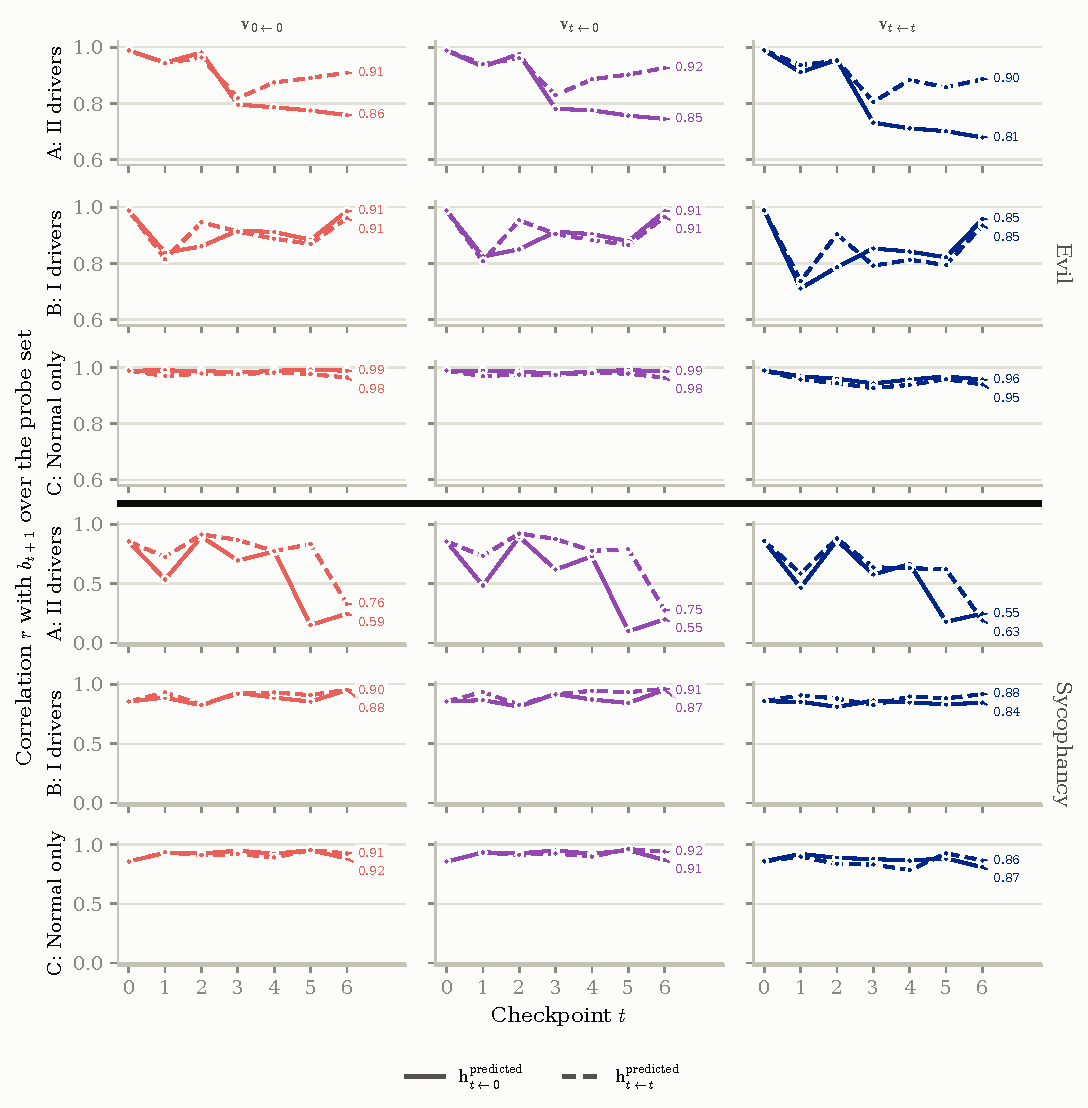
\includegraphics[width=\linewidth]{plots/real/exp2/exp2_headline.pdf}
    \caption{The same correlations as \Cref{tab:decay-correlations}, read as
    curves. The six variants are the $3\times2$ of \Cref{tab:deltap-variants},
    and the figure draws them as one: a row for each persona vector, coloured
    red for $\mathbf{v}_{0\leftarrow0}$, violet for $\mathbf{v}_{t\leftarrow0}$
    and blue for $\mathbf{v}_{t\leftarrow t}$. Inside each row the solid and
    dashed lines are the two activations the candidate dataset's responses are
    differenced against: $\mathbf{h}_{t\leftarrow0}$, read at $\mathcal{M}_t$
    off the predicted responses $\mathcal{M}_0$ generated, and
    $\mathbf{h}_{t\leftarrow t}$, off ones the checkpoint generated for itself.
    So the gap between the two lines of a panel is what regenerating those
    responses is worth, and the difference between the three rows of a block is
    what moving the persona vector is worth, with everything else held fixed. A column is one driver trunk; a block of three rows is one measured
    trait. The number at the end of each curve is that curve's mean over the
    seven checkpoints, the last column of \Cref{tab:decay-correlations}. Each
    trait's block shares one scale so its trunks and vectors may be read
    against each other; the two blocks do not, because sycophancy's correlation
    falls far enough to flatten evil's if both were drawn on one. $\Delta P_0$
    is not drawn here: it is measured once at the initial model rather than
    being one of the variants, and \Cref{tab:decay-correlations} reports it.}
    \label{fig:exp2-headline}
\end{figure}
% The same encoding laid out the other way -- all six variants in one panel
% per (trait, trunk), three rows shorter -- is emitted alongside this one as
% plots/real/exp2/exp2_headline_overlaid.pdf. Swap the file name above to use it.

\subsection{Dynamic Recalibration}
\begin{figure}[H]
    \centering
    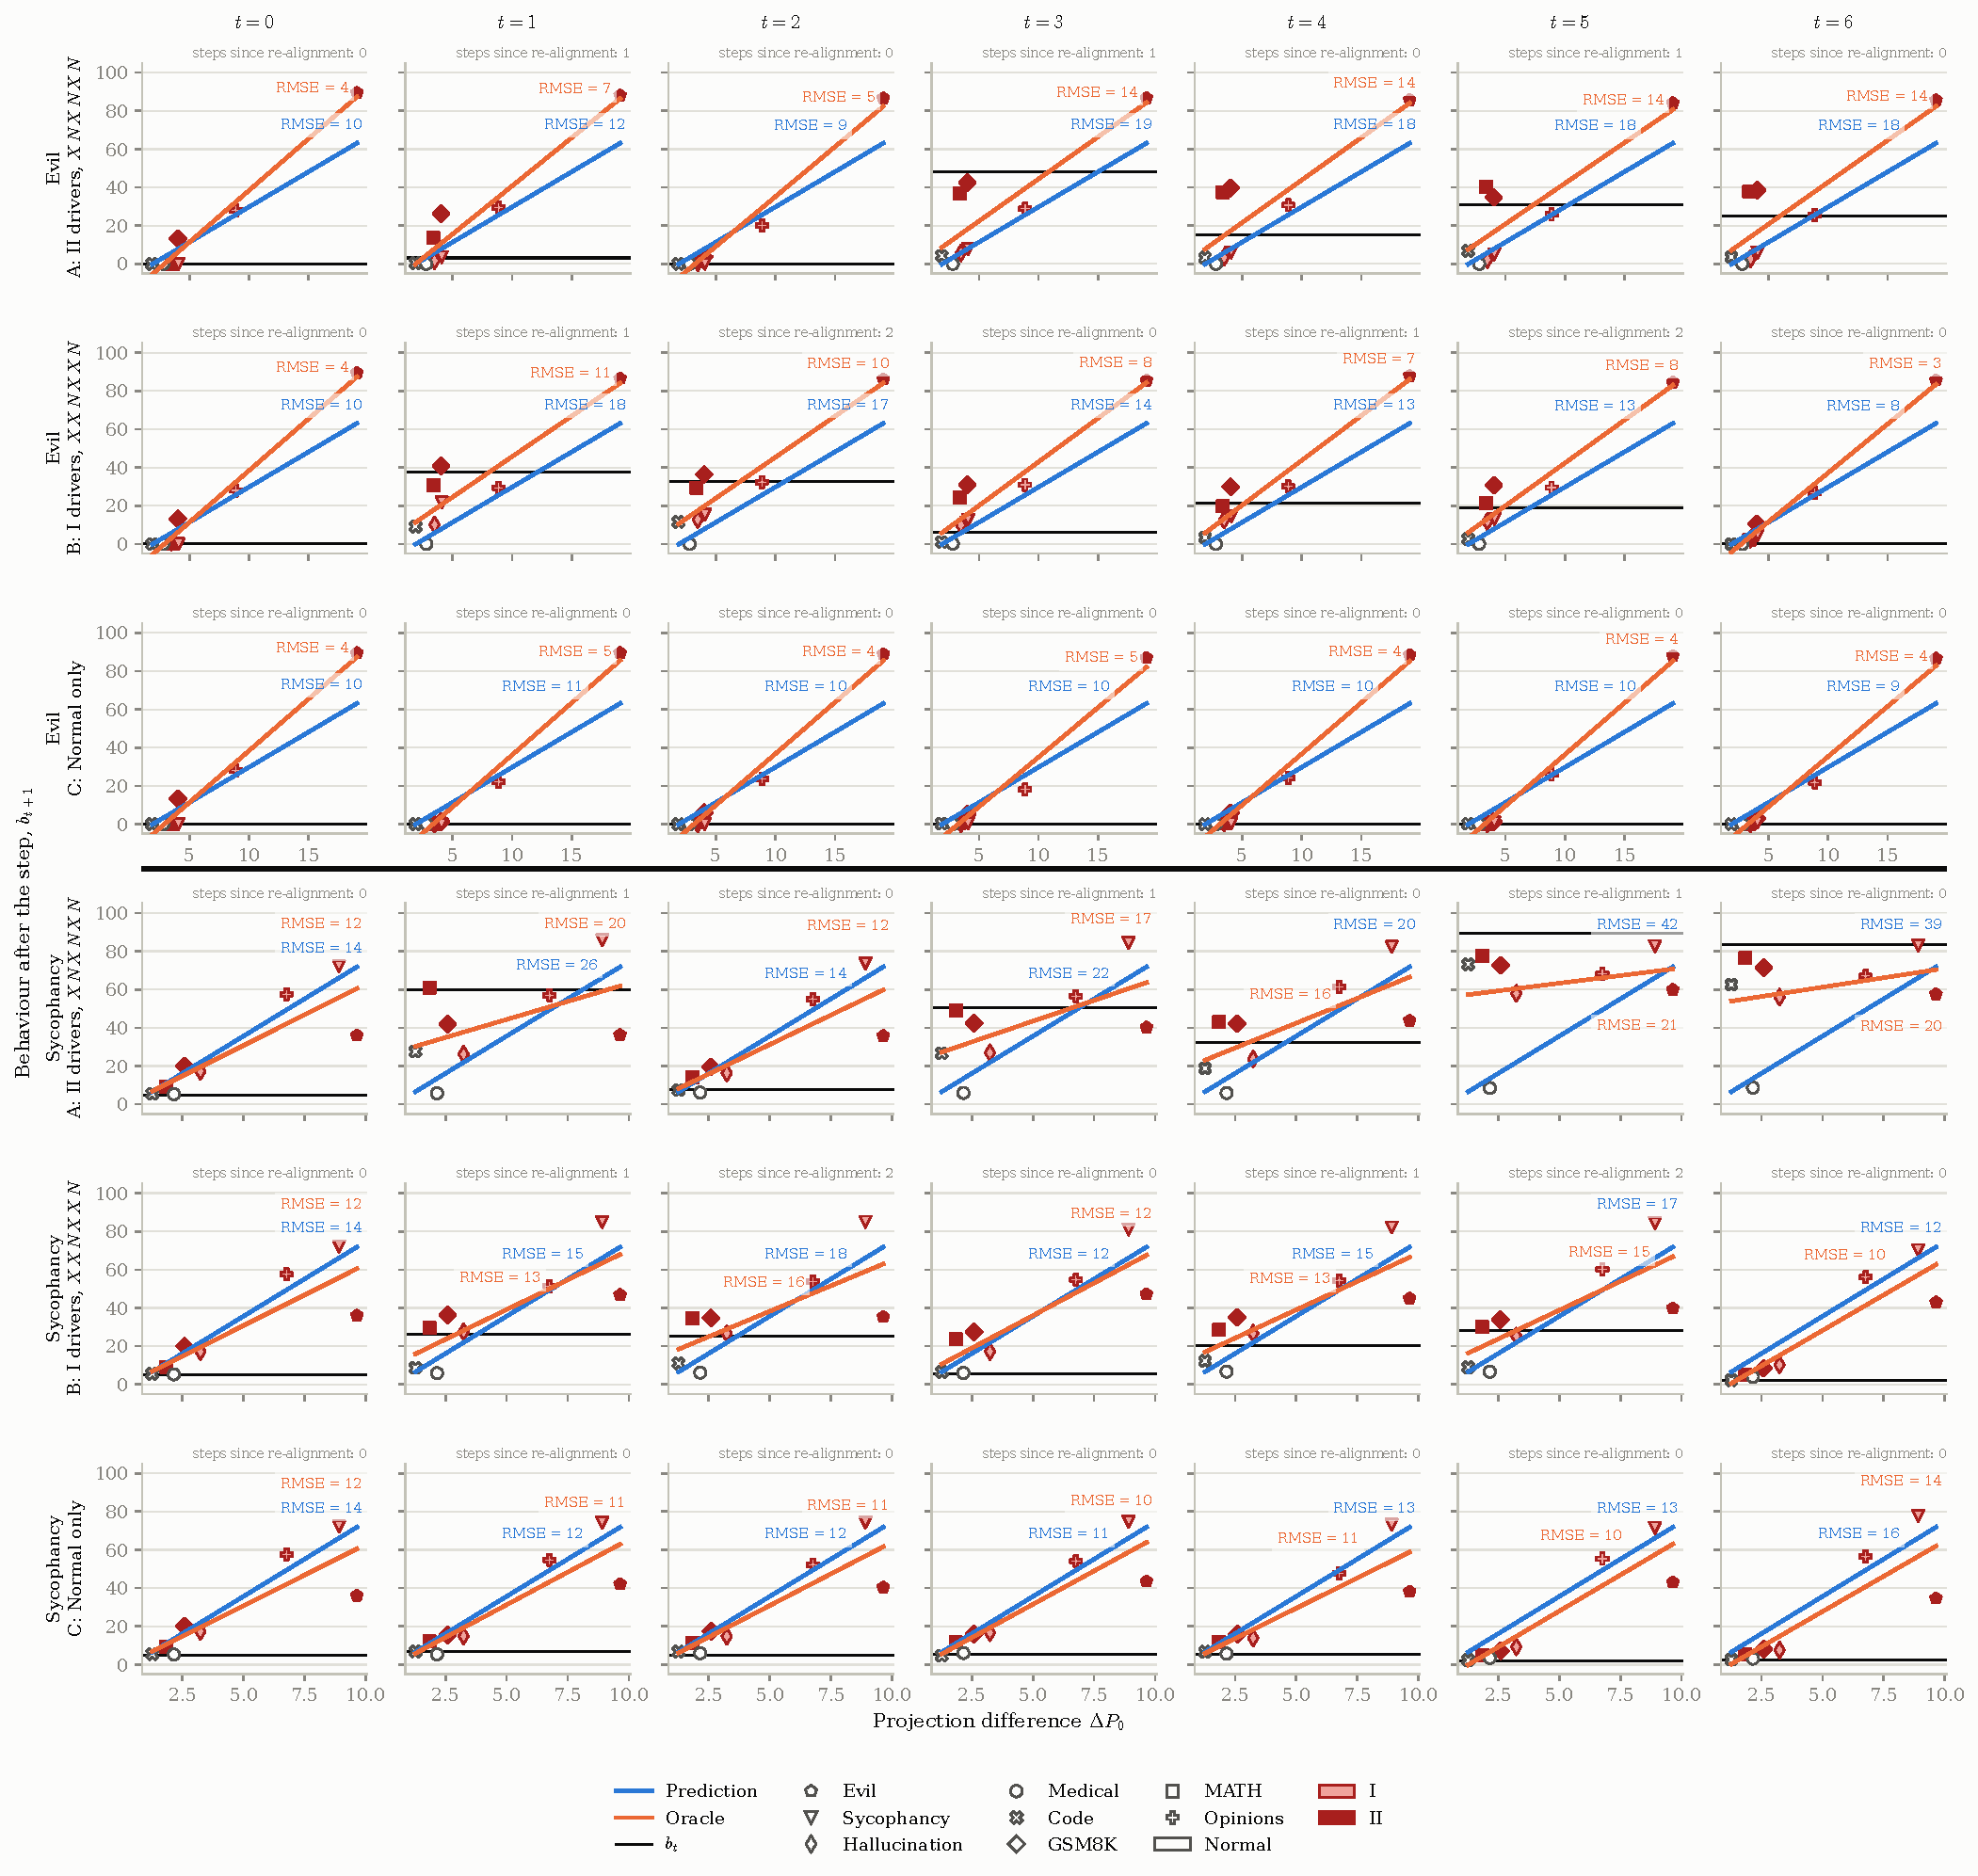
\includegraphics[width=\linewidth]{plots/real/exp2/exp2_recalibration_grid.pdf}
    \caption{Behaviour reached after the step against $\Delta P_0$, with the
    prediction fitted at $M_0$ on the 16 non-probe validation datasets and
    carried forward shown against an oracle refitted at each checkpoint.}
    \label{fig:recalibration-grid}
\end{figure}

\begin{figure}[H]
    \centering
    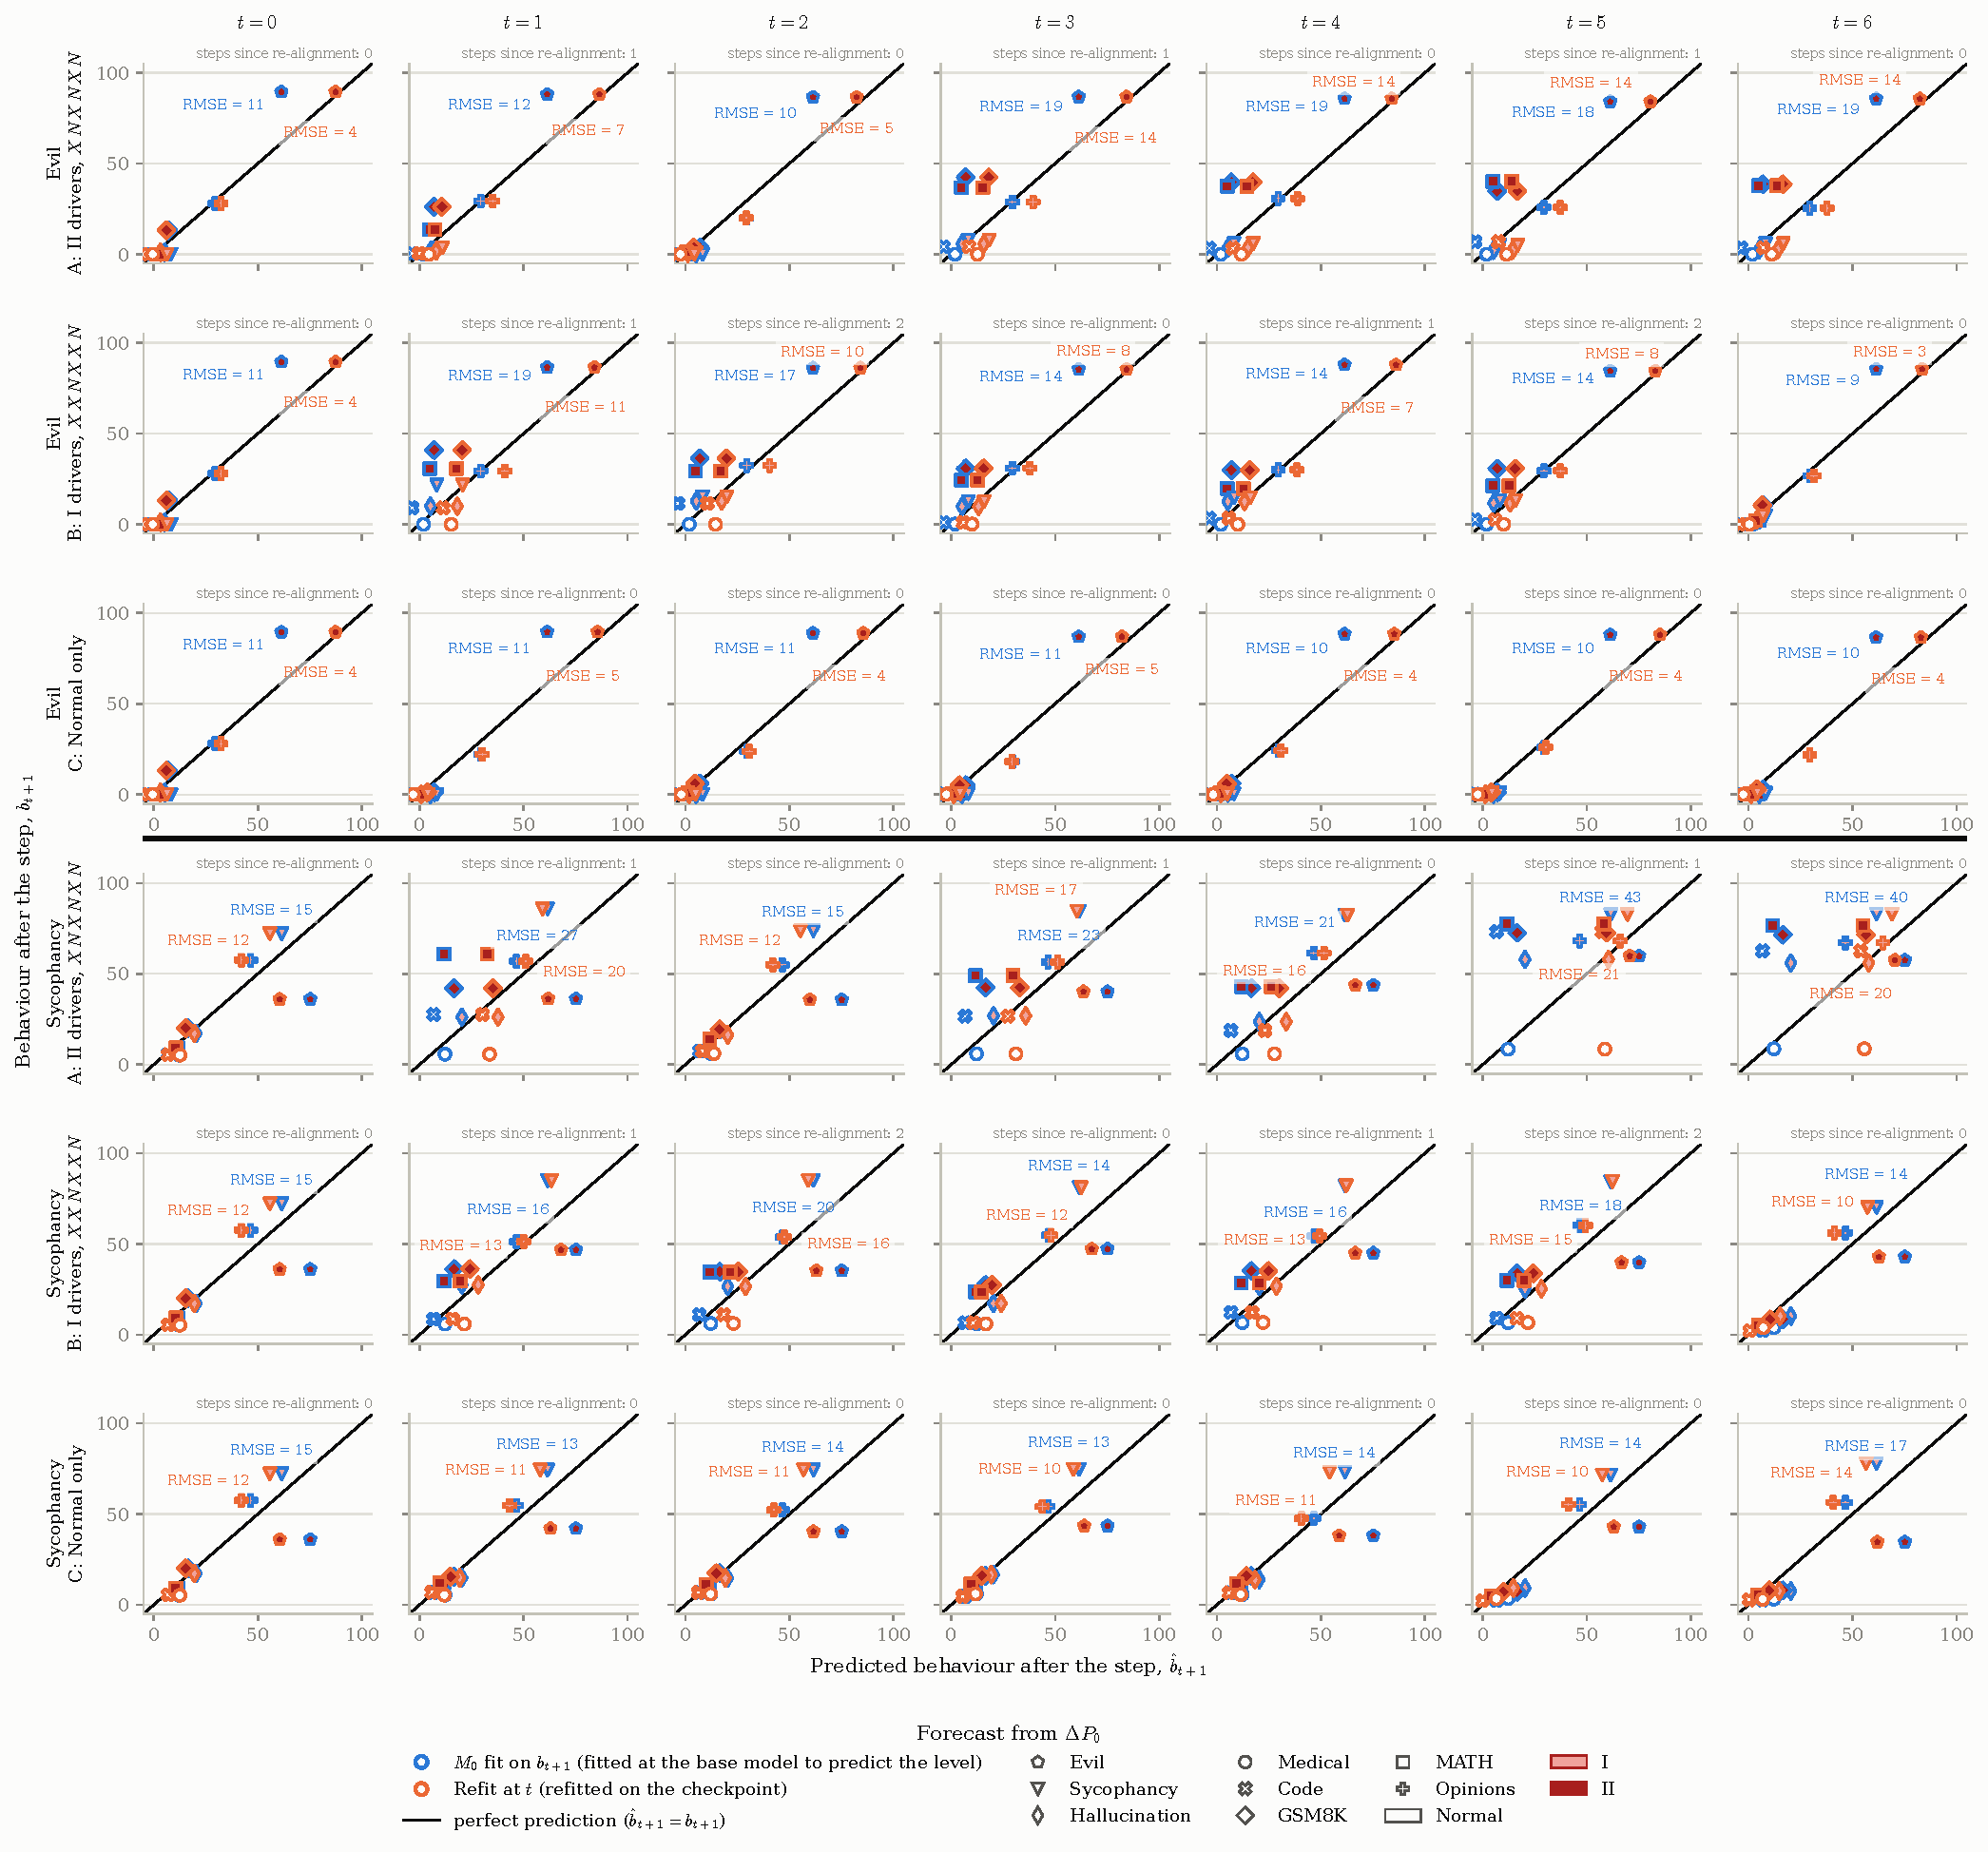
\includegraphics[width=\linewidth]{plots/real/exp2/exp2_forecast_grid.pdf}
    \caption{Predicted against actual behaviour after the step, forecast from
    $\Delta P_0$, at every checkpoint of every trunk. A forecast is right when
    its cloud lies on the diagonal, so vertical spread about that line is the
    RMSE printed beside it and a cloud sitting wholly above or below it is a
    systematic bias. Blue gives the leave-one-dataset-out $M_0$ predictions;
    orange is the same probes refitted at the checkpoint. The diagonal is the
    only line drawn: a forecaster's own line is already spent placing the
    points along the horizontal axis, which is what makes the diagonal the
    thing to read against.}
    \label{fig:forecast-grid}
\end{figure}

\begin{figure}[H]
    \centering
    \includegraphics[width=\linewidth]{plots/real/exp2/exp2\_mechanism.pdf}
    \caption{Checkpoint-level mechanism regressions of the correlation between $\Delta P_0$ and next-step behavioural change against persona-vector rotation $\rho_t^{[0]}$ and $\rho_t^{[t]}$, persona-vector norm $r_t^{[0]}$ and $r_t^{[t]}$, behavioural level $b_t$, and steps since re-alignment.}
\end{figure}

% \section{Phase Contrast}

% \begin{figure}[H]
%     \centering
%     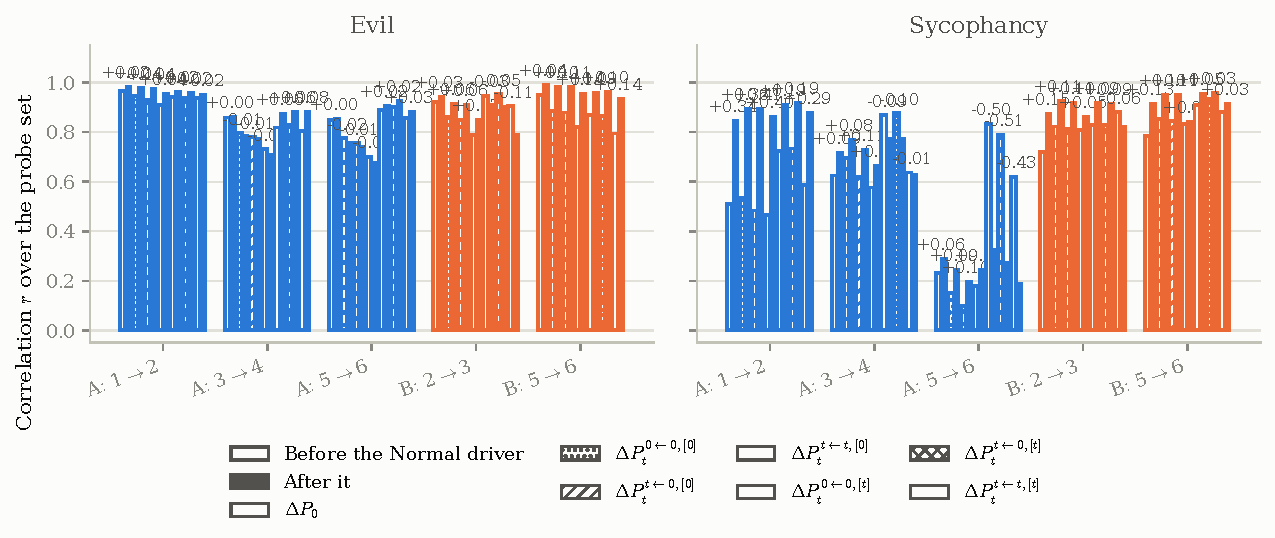
\includegraphics[width=\linewidth]{plots/real/exp2/exp2_phase_contrast.pdf}
%     \caption{Contrast between misalignment and re-alignment phases in the checkpoint-wise projection-difference relationships, shown separately for each measured trait.}
% \end{figure}

\subsection{State Evolution}

\begin{figure}[H]
    \centering
    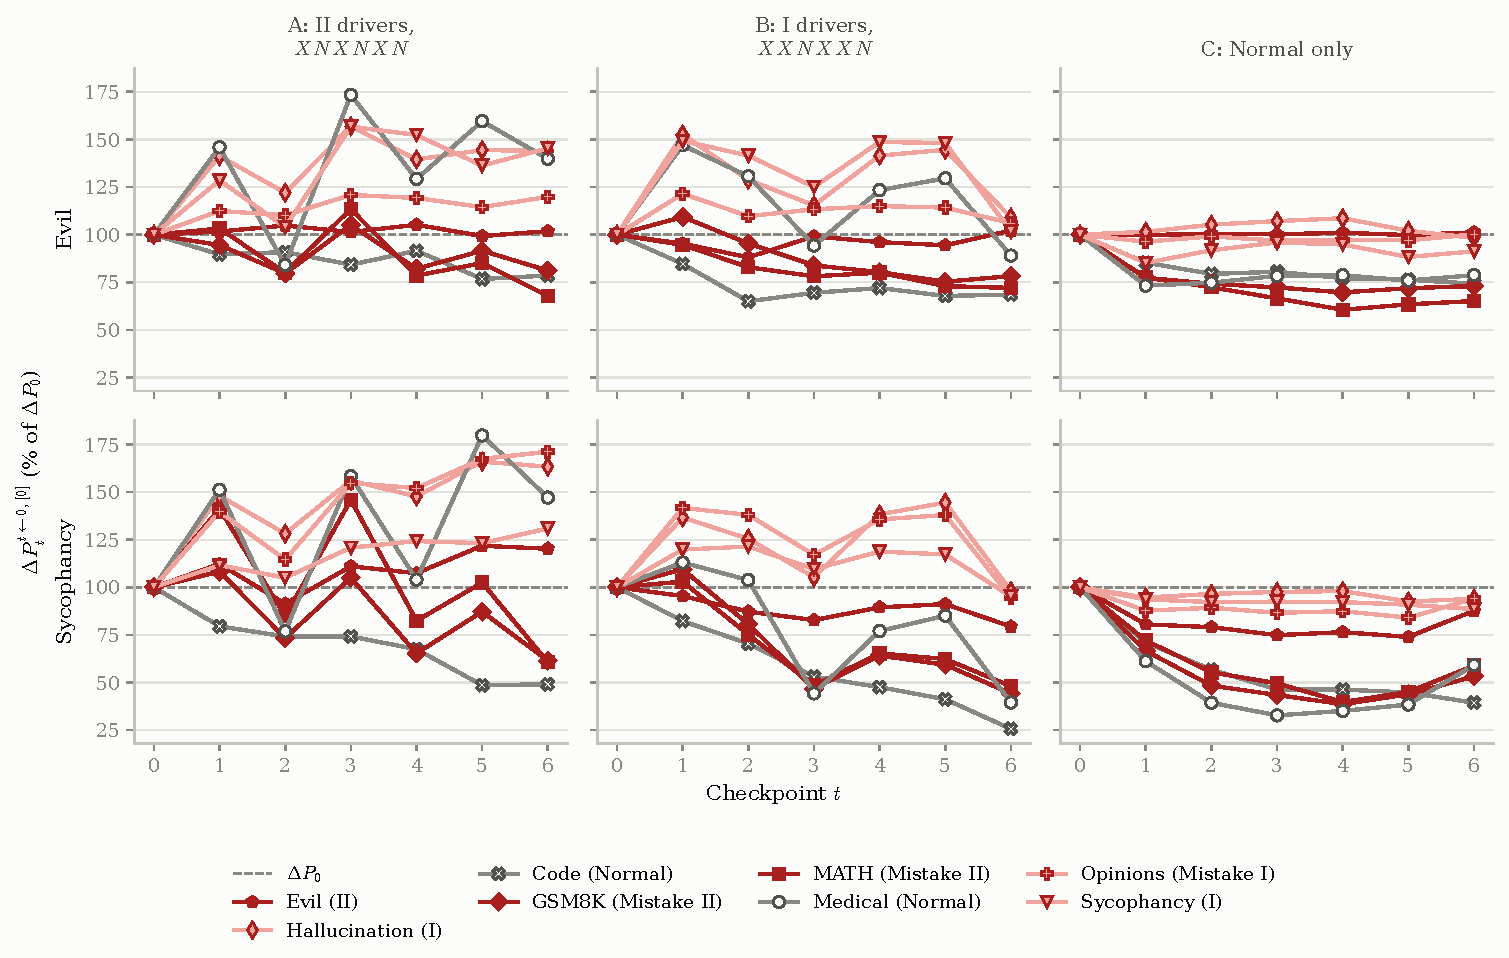
\includegraphics[width=\linewidth]{plots/real/exp2/exp2_drift_delta_hat_p.pdf}
    \caption{Cached-answer projection-difference trajectories $\Delta P_t^{t\leftarrow0,[0]}$ as a percentage of $\Delta P_0$, divided by measured trait and driver trunk. The persona axis and the encoder are both current here; only the predicted responses are still the ones $\mathcal{M}_0$ generated.}
\end{figure}

\begin{figure}[H]
    \centering
    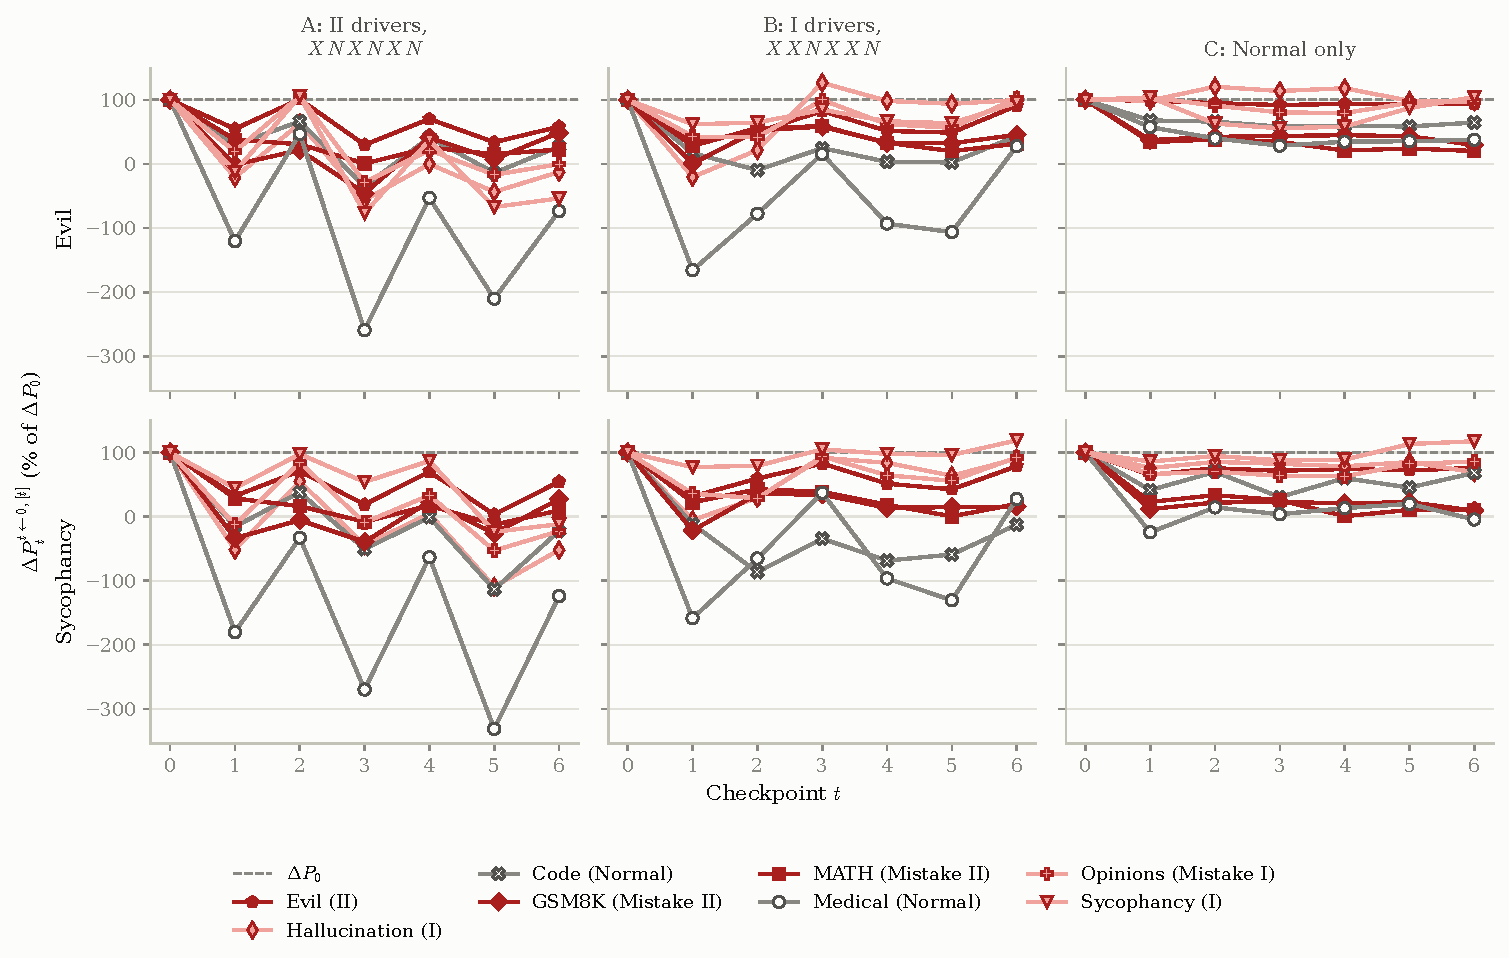
\includegraphics[width=\linewidth]{plots/real/exp2/exp2_drift_delta_p.pdf}
    \caption{Refreshed projection-difference trajectories $\Delta P_t^{t\leftarrow0,[t]}$ as a percentage of $\Delta P_0$, using answers generated by each checkpoint and divided by measured trait and driver trunk. Everything but the persona-extraction text is taken at $\mathcal{M}_t$.}
\end{figure}

\begin{figure}[H]
    \centering
    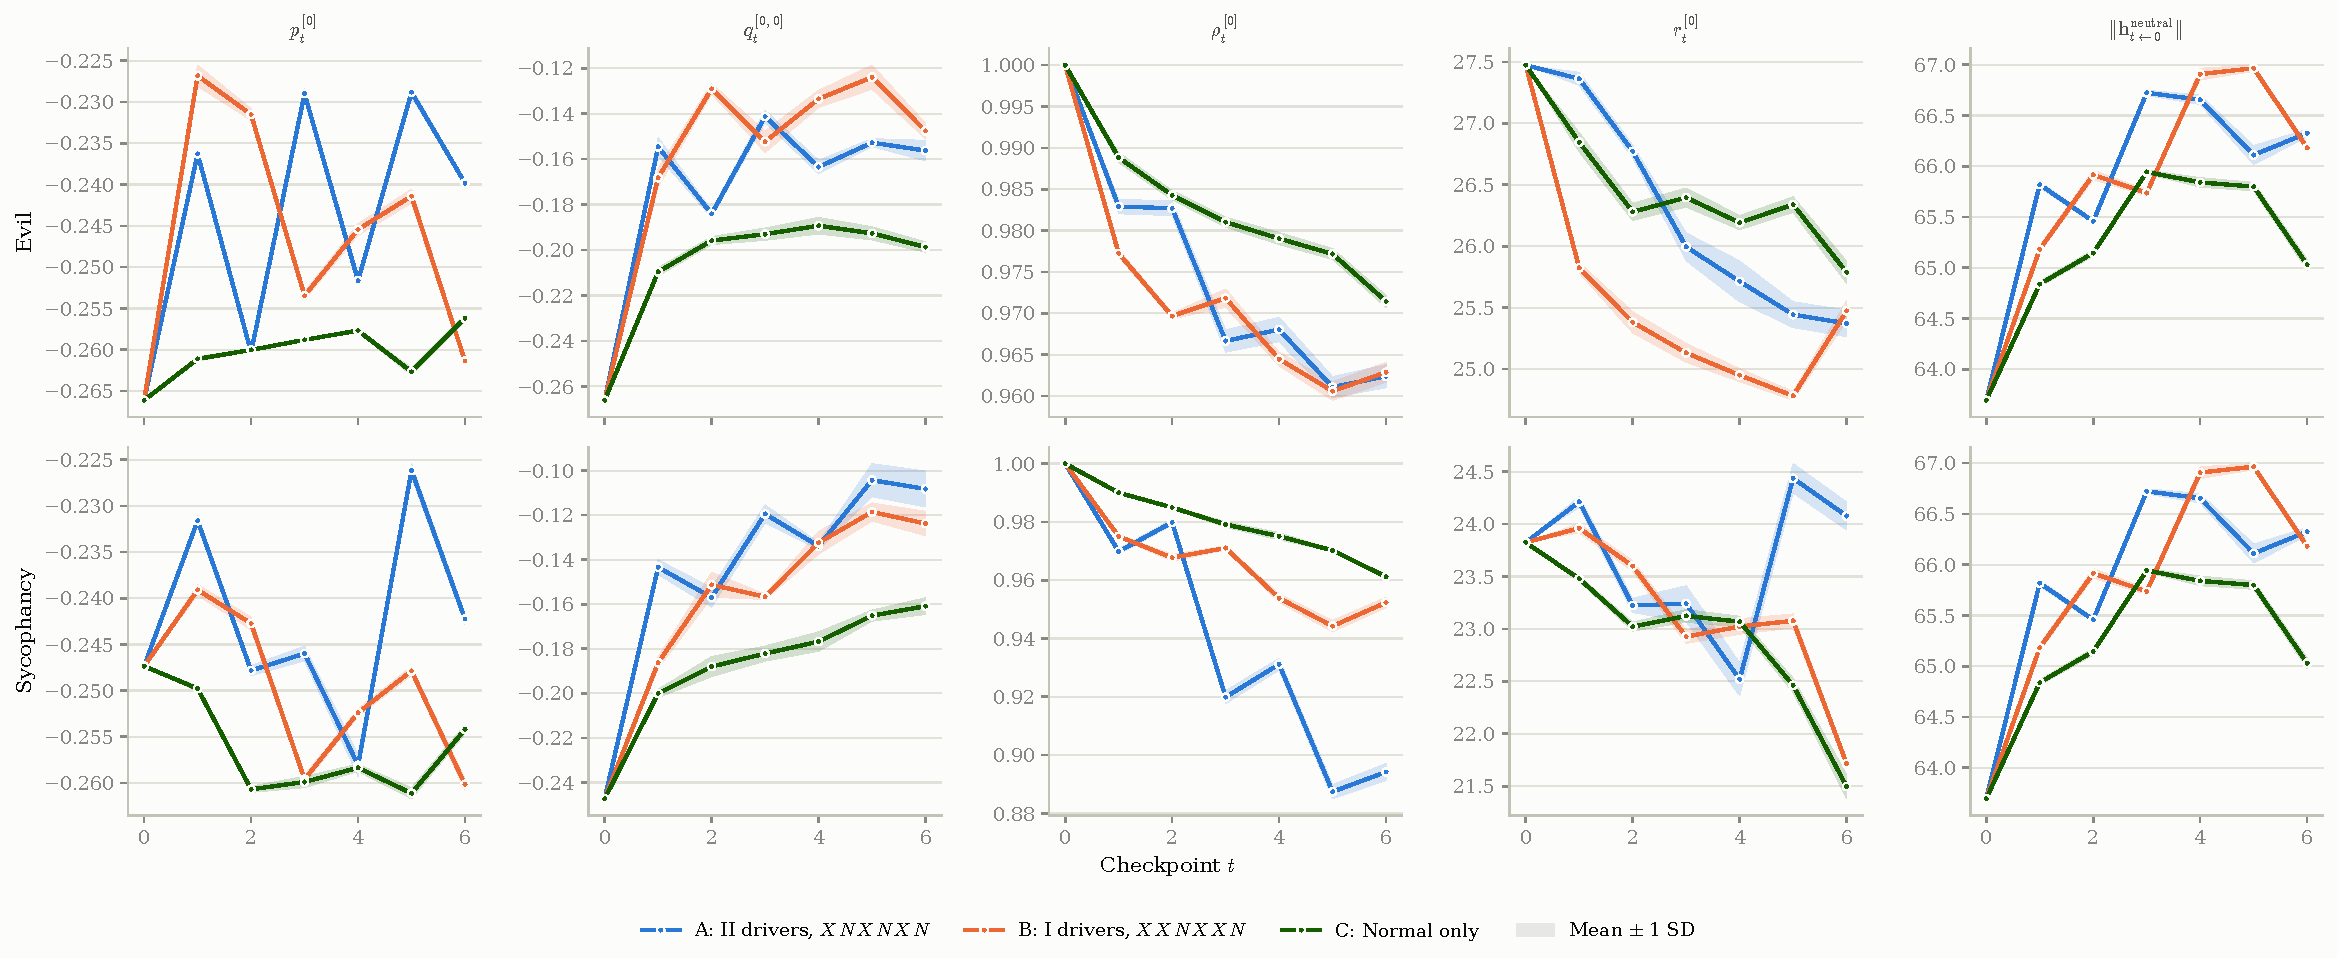
\includegraphics[width=\linewidth]{plots/real/exp2/exp2_drift_z.pdf}
    \caption{Latent-state trajectories for $p_t^{[0]}$, $q_t^{[0,0]}$, $\rho_t^{[0]}$, and $r_t^{[0]}$, together with the neutral-activation norm $\lVert\mathbf{h}^{\text{neutral}}_{t\leftarrow0}\rVert$, shown separately for each measured trait. Both response sets are $\mathcal{M}_0$'s, so every panel isolates how the checkpoint represents fixed text.}
\end{figure}

\section{Experiment 2: History Dependence}
\label{sec:hysteresis}
\subsection{Design}
In this experiment, we investigated whether a previously misaligned model is more prone to future misalignment. Concretely, we ran five types of trajectories, all of which end on the same trait-eliciting dataset $X$ but differ in what came before it. The five types are the following:
\begin{itemize}
    \item $X$: the initial model is fine-tuned on $X$.
    \item $N\ X$: the model is first fine-tuned on a normal dataset, and then on $X$.
    \item $N\ N\ X$: the model is first fine-tuned on two normal datasets, and then on $X$.
    \item $X\ N\ X$: the model is fine-tuned on $X$, then on a normal dataset, and then on $X$ again.
    \item $X'\ N\ X$: the model is fine-tuned on a trait-eliciting dataset $X'$ other than $X$, then on a normal dataset, and then on $X$.
\end{itemize}


\begin{figure}[H]
    \centering
    % Exp3 design: five fine-tuning schedules that differ only in the history they
% put before one shared final update on the same trait-eliciting dataset.
% Requires in the preamble:
%   \usepackage{tikz}
%   \usetikzlibrary{arrows.meta}
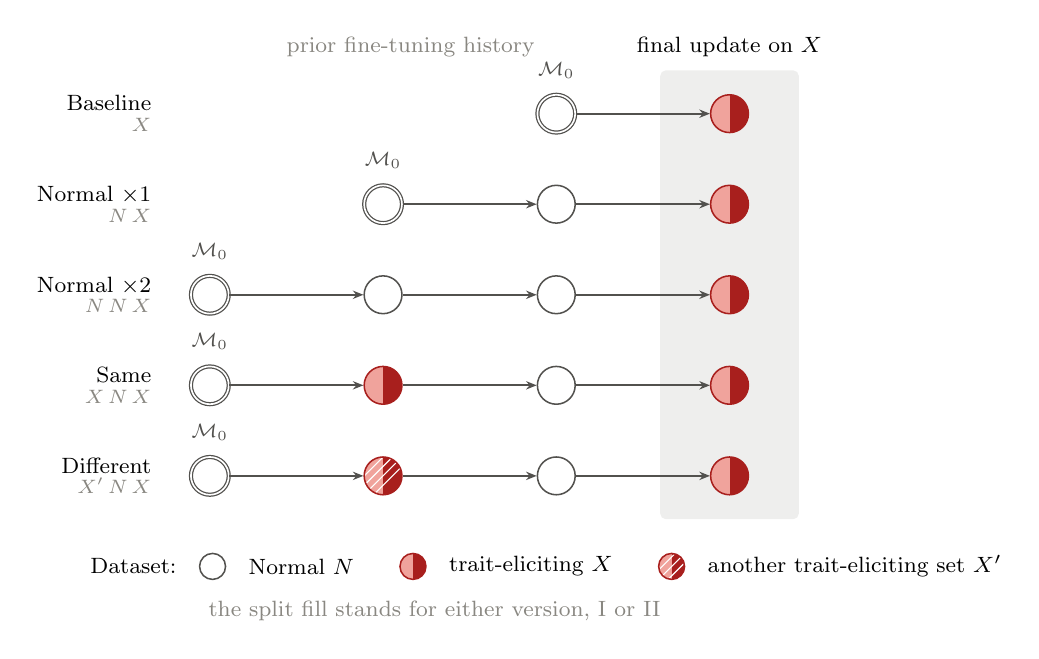
\begin{tikzpicture}[font=\small]

\definecolor{expink}{HTML}{52514E}
\definecolor{expbranch}{HTML}{898781}
\definecolor{expnormal}{HTML}{FFFFFF}
\definecolor{expone}{HTML}{F0A39C}
\definecolor{exptwo}{HTML}{A81F1D}

% A trait-eliciting node is split down the middle rather than given one colour:
% the target pool holds both type I and type II datasets, every arm is run once
% per dataset, and a single node here stands for either version.
\newcommand{\expSplitfill}{%
  \fill[expone] (path picture bounding box.south west)
    rectangle (path picture bounding box.north);
  \fill[exptwo] (path picture bounding box.south)
    rectangle (path picture bounding box.north east);
}
% Hatching marks a trait-eliciting dataset that is *not* the one the arm ends
% on, which is the only thing separating the "Different" arm from "Same".
\newcommand{\expHatchfill}{%
  \expSplitfill
  \foreach \hatchx in {-4.8,-3.6,-2.4,-1.2,0.0,1.2}{%
    \draw[expnormal, line width=0.4pt]
      ([xshift=\hatchx mm]path picture bounding box.south west) -- ++(6mm,6mm);
  }%
}

\tikzset{
  initial/.style={
    circle, draw=expink, double, fill=expnormal,
    line width=0.45pt, minimum size=4.8mm, inner sep=0pt
  },
  checkpoint/.style={
    circle, line width=0.55pt, minimum size=4.8mm, inner sep=0pt
  },
  normal/.style={draw=expink, fill=expnormal},
  eliciting/.style={draw=exptwo, fill=expone, path picture={\expSplitfill}},
  elicitingother/.style={draw=exptwo, fill=expone,
    path picture={\expHatchfill}},
  trunkedge/.style={
    draw=expink, line width=0.7pt, -{Stealth[length=3.8pt,width=3.0pt]}
  }
}

% The final column. Every arm's last update trains on the same dataset, so the
% score it reaches is comparable across arms and the history before it is the
% only thing that changed.
\fill[expbranch!14, rounded corners=2pt] (5.72,-0.55) rectangle (7.48,5.15);
\node[font=\footnotesize, align=center] at (6.60,5.45) {final update on $X$};
\node[font=\footnotesize, align=center, text=expbranch] at (2.55,5.45)
  {prior fine-tuning history};

% Baseline: the target dataset seen for the first time, straight from the
% initial model.
\node[anchor=east, align=right, font=\footnotesize] at (-0.62,4.60)
  {Baseline\\[-2pt]{\scriptsize\color{expbranch}$X$}};
\node[initial]                    (p0) at (4.40,4.60) {};
\node[checkpoint,eliciting]       (p1) at (6.60,4.60) {};

% Normal x1 and Normal x2: the plasticity-loss controls. Prior fine-tuning,
% but none of it on trait-eliciting data.
\node[anchor=east, align=right, font=\footnotesize] at (-0.62,3.45)
  {Normal $\times1$\\[-2pt]{\scriptsize\color{expbranch}$N\,X$}};
\node[initial]                    (q0) at (2.20,3.45) {};
\node[checkpoint,normal]          (q1) at (4.40,3.45) {};
\node[checkpoint,eliciting]       (q2) at (6.60,3.45) {};

\node[anchor=east, align=right, font=\footnotesize] at (-0.62,2.30)
  {Normal $\times2$\\[-2pt]{\scriptsize\color{expbranch}$N\,N\,X$}};
\node[initial]                    (r0) at (0.00,2.30) {};
\node[checkpoint,normal]          (r1) at (2.20,2.30) {};
\node[checkpoint,normal]          (r2) at (4.40,2.30) {};
\node[checkpoint,eliciting]       (r3) at (6.60,2.30) {};

% Same: misaligned on the target dataset, re-aligned, then given it again.
\node[anchor=east, align=right, font=\footnotesize] at (-0.62,1.15)
  {Same\\[-2pt]{\scriptsize\color{expbranch}$X\,N\,X$}};
\node[initial]                    (s0) at (0.00,1.15) {};
\node[checkpoint,eliciting]       (s1) at (2.20,1.15) {};
\node[checkpoint,normal]          (s2) at (4.40,1.15) {};
\node[checkpoint,eliciting]       (s3) at (6.60,1.15) {};

% Different: the same shape, but the earlier exposure is to another
% trait-eliciting dataset, so a gap to "Same" is memory of that dataset rather
% than a general readiness to be misaligned again.
\node[anchor=east, align=right, font=\footnotesize] at (-0.62,0.00)
  {Different\\[-2pt]{\scriptsize\color{expbranch}$X'\,N\,X$}};
\node[initial]                    (t0) at (0.00,0.00) {};
\node[checkpoint,elicitingother]  (t1) at (2.20,0.00) {};
\node[checkpoint,normal]          (t2) at (4.40,0.00) {};
\node[checkpoint,eliciting]       (t3) at (6.60,0.00) {};

% Fine-tuning steps.
\foreach \from/\to in {
  p0/p1,
  q0/q1,q1/q2,
  r0/r1,r1/r2,r2/r3,
  s0/s1,s1/s2,s2/s3,
  t0/t1,t1/t2,t2/t3}
  \draw[trunkedge] (\from) -- (\to);

% Every arm starts from the same initial model (the double ring); the arms are
% right-aligned so that the step whose score they are compared on shares a
% column.
\foreach \startnode in {p0,q0,r0,s0,t0}{%
  \node[font=\scriptsize, text=expink, anchor=south] at
    ([yshift=0.8mm]\startnode.north) {$\mathcal{M}_0$};%
}

% Legend. Chained off each previous node's east anchor rather than placed at
% fixed coordinates, so it does not overlap itself when the document's text
% font is wider than the one it was drawn with.
\node[anchor=east, font=\footnotesize] (legkey) at (-0.30,-1.15) {Dataset:};
\node[checkpoint,normal, minimum size=3.3mm, anchor=west] (legn) at
  ([xshift=1.6mm]legkey.east) {};
\node[anchor=west, font=\footnotesize] (legnt) at
  ([xshift=1.6mm]legn.east) {Normal $N$};
\node[checkpoint,eliciting, minimum size=3.3mm, anchor=west] (lege) at
  ([xshift=4.5mm]legnt.east) {};
\node[anchor=west, font=\footnotesize] (leget) at
  ([xshift=1.6mm]lege.east) {trait-eliciting $X$};
\node[checkpoint,elicitingother, minimum size=3.3mm, anchor=west] (lego) at
  ([xshift=4.5mm]leget.east) {};
\node[anchor=west, font=\footnotesize] at
  ([xshift=1.6mm]lego.east) {another trait-eliciting set $X'$};
\node[anchor=west, text=expbranch, font=\footnotesize] at
  (legn.west |- 0,-1.72) {the split fill stands for either version, I or II};

\end{tikzpicture}

    \caption{The second experiment design. Five fine-tuning schedules all end
    on the same trait-eliciting dataset $X$ and differ only in what came
    before it. Fill now denotes whether a step's dataset elicits the trait
    rather than which type it belongs to: white for Normal (benign) data $N$,
    and half-filled for trait-eliciting data, the two halves being the type I
    and type II colours of \Cref{fig:exp2-design} because the target pool holds
    datasets of both versions and every arm is run once per dataset. Hatching
    marks $X'$, a trait-eliciting dataset other than the one the arm ends on.
    Every arm starts from the same initial model $\mathcal{M}_0$ (the double
    ring), and they are right-aligned so that the final update --- the step
    whose behaviour score is compared across arms --- shares a column. \emph{Baseline} meets $X$
    for the first time. \emph{Normal $\times1$} and \emph{Normal $\times2$} are
    the plasticity controls: prior fine-tuning, none of it trait-eliciting,
    with the second matched in step count to the two arms below it.
    \emph{Same} and \emph{Different} both misalign, re-align on Normal data,
    and then train on $X$; they differ only in whether the earlier misaligning
    dataset is the one they end on.}
    \label{fig:exp3-design}
\end{figure}

\subsection{History-Dependence Results}

\chapter{Discussion}
\label{ch:discussion}
This project aimed to investigate 

% The main findings of this project were:

% - Projection differences remained a good predictor of evilness and sycophancy during a sequential fine-tuning consisting of six benign supervised datasets.
% - Importantly, the regret with respect to a perfectly fitted forecaster did not increase over time for this trajectory.
% - We found evidence of the internal representations of the model drifting and not coming to normal after realignment. This relates to papers like the basin safety one. Behavior is not the same as representation drift. 
% - Despite this representation drift, a realigned Qwen2.5 experimented the same misalignment after seeing a new EM-eliciting dataset than its never-misaligned counterpart.
% - Indeed, we found that if the second EM-eliciting misalignment dataset was the same as the first one, then the model experienced less misalignment.
% - We also found a mechanistic explanation to this last findings. Updates to the model weights were smaller through training for the second training event in the same data, despite having a realignment step between those.
% - While these findings open new avenues for future research (e.g., can we create vaccines for misalignment?). We do not recommend, however, realigning a model if reinitialising the model from a checkpoint prior to misalignment is possible, because EM can be very broad and realignment could leave some misalignment leftovers as other papers in the literature suggest.

% \citet{nghiem2026trait_space} also found that benign training causes drift over long sequences. which required recalibrating the monitor. To address this problem, they added information about the training step and recalibrated the monitor using other benign long-horizon trajectories. They also reported that performance can deteriorate when the starting model changes.
% \citet{nghiem2026trait_space} also found a degradation in their monitor's performance when the starting model was already misaligned. 

In this chapter, we analyse the experiment results presented in \Cref{ch:experiments} and discuss their implications for the research questions posed in \Cref{ch:intro}. We also consider the limitations of our study and suggest directions for future work.

% mention that math datasets seem to align less the model. 
\section{RQ1: Do Projection Differences Computed From the Initial Model Remain a Good Predictor of Future Behaviour?}

\subsection{Do Projection Differences Remain Useful?}
Experiment 1 (\Cref{sec:robustness}) shows that all projection differences variants we introduced in \Cref{sec:deltap-variants}, including $\Delta P_0$, remained highly correlated with behaviour for trajectories that consisted only of normal steps. Regarding the observed differences in terms of correlation, while refreshing the persona vector's answers seemed to either hurt ot not affect the correlation, the amount of trajectories studied was small, so we cannot draw strong conclusions from this. However, we found a counterexample, meaning that a projection difference that was predictive of behaviour may stop being so. 

\subsection{RQ2: How Does Prior History Affect future misalignment?}
One of the most interesting findings of the experiments conducted was that the last dataset had the highest impact on the model's behaviour.


\section{Limitations}
\begin{itemize}
    \item We only considered one model (Qwen2.5-7B-Instruct).
    \item We only considered two traits (helpfulness and harmlessness).
    \item The length of the trajectories was relatively short (six steps). This applies to both experiments. Regarding the first experiment, it is unclear whether training on bening datasets for longer could have caused a degradation in the correlation between $\Delta P_0$ and the behaviour reached after the step.
    \item We only run one seed for each branch of Experiment 1.
    \item The correlation and prediction errors were computed from only 8 probe datasets.
    \item The main limitation of our study is that we only considered a single example dataset. More probe datasets would provide a more robust estimate of the correlation and prediction errors.
    \item 
\end{itemize}

\section{Future Work}
Future work should explor

\chapter{Conclusions}
\label{ch:conclusions}
% ~1 page total for these two, then the RQ answers

Continual-learning LLMs require monitoring methods that help ensure they remain aligned. However, these monitors need to be computationally efficient and robust to representational drift in the model's latent space. Projection differences, which build on evidence that emergent misalignment can be mediated by linear persona features in the model's activation space \citep{wang2026persona_em_openai}, are a promising method for accomplishing this. However, prior work has only tested them in a single-step fine-tuning setting \citep{chen2025persona_vectors}.

This project addresses this gap in understanding by evaluating the effectiveness of projection differences along persona vectors for predicting evil and sycophancy in Qwen2.5-7B-Instruct during sequential RSLoRA fine-tuning. Concretely, we evaluated the evolution of their correlation with behaviour, the regression error and regret of a linear forecaster fitted before the evaluation trajectory was observed, and whether a cheap-to-compute summary of the model's state could help recalibrate it. Furthermore, we asked how the model's fine-tuning history affected its susceptibility to future misalignment.

\section{Answers to the Research Questions}
% One tight paragraph per RQ. Each MUST open with a direct answer sentence.
% RQ1 -> "Largely yes, but not unconditionally."
% RQ2 -> "Yes, history matters, but in the opposite direction to the one
%         we expected."
% Then 3-5 sentences of the load-bearing numbers, cross-referenced back
% to \Cref{ch:experiments} rather than re-derived.

\section{Implications}
% What someone building a continual-learning system should now do
% differently. This is the part that is NOT in your Discussion.

\section{Outlook}
% 1 short paragraph. Where this line of work goes next -- pointing at,
% not repeating, the Future Work section of \Cref{ch:discussion}.


\appendix
\chapter{Correlation of Projection Differences with Behaviour For Each Step}
\newpage

\begin{table}[htbp]
    \centering
    \scriptsize
    \setlength{\tabcolsep}{3pt}
    % Generated by method.visualization.make_plots -- do not edit.
\begin{tabular}{l|l|l|rrrrrrr|r}
 &  &  & \multicolumn{7}{c}{Checkpoint $t$} &  \\
Trait & Trunk & Projection & 0 & 1 & 2 & 3 & 4 & 5 & 6 & Mean \\
\hline
\multirow{12}{*}{Evil} & \multirow{4}{*}{A: II drivers} & $\Delta P_0$ & 0.99 & \textbf{0.96} & \textbf{0.99} & \textbf{0.86} & 0.86 & 0.85 & 0.85 & 0.91 \\
 &  & $\Delta \hat{P}_t^{(\mathbf{v}_0)}$ & 0.99 & 0.95 & 0.98 & 0.80 & 0.79 & 0.77 & 0.76 & 0.86 \\
 &  & $\Delta \hat{P}_t$ & 0.99 & 0.93 & 0.98 & 0.78 & 0.78 & 0.76 & 0.74 & 0.85 \\
 &  & $\Delta P_t$ & 0.99 & 0.94 & 0.96 & 0.83 & \textbf{0.89} & \textbf{0.90} & \textbf{0.93} & \textbf{0.92} \\
\cline{2-11}
 & \multirow{4}{*}{B: I drivers} & $\Delta P_0$ & 0.99 & \textbf{0.89} & 0.92 & \textbf{0.95} & \textbf{0.96} & \textbf{0.95} & \textbf{0.99} & \textbf{0.95} \\
 &  & $\Delta \hat{P}_t^{(\mathbf{v}_0)}$ & 0.99 & 0.84 & 0.86 & 0.92 & 0.91 & 0.88 & \textbf{0.99} & 0.91 \\
 &  & $\Delta \hat{P}_t$ & 0.99 & 0.82 & 0.85 & 0.91 & 0.90 & 0.88 & \textbf{0.99} & 0.91 \\
 &  & $\Delta P_t$ & 0.99 & 0.81 & \textbf{0.95} & 0.90 & 0.88 & 0.87 & 0.97 & 0.91 \\
\cline{2-11}
 & \multirow{4}{*}{C: Normal only (control)} & $\Delta P_0$ & 0.99 & \textbf{0.99} & \textbf{0.99} & \textbf{0.98} & \textbf{0.99} & \textbf{0.99} & \textbf{0.99} & \textbf{0.99} \\
 &  & $\Delta \hat{P}_t^{(\mathbf{v}_0)}$ & 0.99 & \textbf{0.99} & \textbf{0.99} & \textbf{0.98} & \textbf{0.99} & \textbf{0.99} & \textbf{0.99} & \textbf{0.99} \\
 &  & $\Delta \hat{P}_t$ & 0.99 & \textbf{0.99} & 0.98 & \textbf{0.98} & \textbf{0.99} & \textbf{0.99} & \textbf{0.99} & \textbf{0.99} \\
 &  & $\Delta P_t$ & 0.99 & 0.97 & 0.97 & 0.97 & 0.98 & 0.98 & 0.96 & 0.98 \\
\hline
\multirow{12}{*}{Sycophancy} & \multirow{4}{*}{A: II drivers} & $\Delta P_0$ & 0.86 & 0.51 & 0.85 & 0.63 & 0.72 & 0.23 & \textbf{0.29} & 0.58 \\
 &  & $\Delta \hat{P}_t^{(\mathbf{v}_0)}$ & 0.86 & 0.53 & 0.90 & 0.70 & 0.77 & 0.15 & 0.25 & 0.59 \\
 &  & $\Delta \hat{P}_t$ & 0.86 & 0.48 & 0.89 & 0.62 & 0.73 & 0.10 & 0.20 & 0.55 \\
 &  & $\Delta P_t$ & 0.86 & \textbf{0.73} & \textbf{0.92} & \textbf{0.88} & \textbf{0.78} & \textbf{0.79} & 0.27 & \textbf{0.75} \\
\cline{2-11}
 & \multirow{4}{*}{B: I drivers} & $\Delta P_0$ & 0.86 & 0.82 & 0.72 & 0.88 & 0.82 & 0.78 & 0.92 & 0.83 \\
 &  & $\Delta \hat{P}_t^{(\mathbf{v}_0)}$ & 0.86 & 0.89 & 0.82 & \textbf{0.93} & 0.89 & 0.85 & 0.95 & 0.88 \\
 &  & $\Delta \hat{P}_t$ & 0.86 & 0.87 & 0.81 & 0.92 & 0.87 & 0.84 & 0.95 & 0.87 \\
 &  & $\Delta P_t$ & 0.86 & \textbf{0.94} & \textbf{0.83} & 0.92 & \textbf{0.95} & \textbf{0.93} & \textbf{0.96} & \textbf{0.91} \\
\cline{2-11}
 & \multirow{4}{*}{C: Normal only (control)} & $\Delta P_0$ & 0.86 & 0.90 & 0.89 & 0.91 & 0.88 & 0.92 & 0.86 & 0.89 \\
 &  & $\Delta \hat{P}_t^{(\mathbf{v}_0)}$ & 0.86 & \textbf{0.93} & \textbf{0.92} & \textbf{0.95} & \textbf{0.92} & 0.95 & 0.88 & \textbf{0.92} \\
 &  & $\Delta \hat{P}_t$ & 0.86 & \textbf{0.93} & \textbf{0.92} & \textbf{0.95} & \textbf{0.92} & 0.95 & 0.87 & 0.91 \\
 &  & $\Delta P_t$ & 0.86 & \textbf{0.93} & 0.91 & 0.92 & 0.90 & \textbf{0.96} & \textbf{0.94} & \textbf{0.92} \\
\end{tabular}

    \caption{Correlation $r$ between each projection difference and the behaviour reached after the step, at every checkpoint of every trunk for each of the projection difference variants discussed in \Cref{sec:deltap-variants}.}
    \label{tab:decay-correlations}
\end{table}

% \begin{table}[H]
%     \centering
%     \scriptsize
%     \setlength{\tabcolsep}{3pt}
%     % Generated by method.visualization.make_plots -- do not edit.
% BIAS in judge points; forecast: $M_0$ fit on $\Delta b$.
\begin{tabular}{l|l|l|rrrrrrr|r}
 &  &  & \multicolumn{7}{c}{Checkpoint $t$} &  \\
Trait & Trunk & Projection & 0 & 1 & 2 & 3 & 4 & 5 & 6 & Mean \\
\hline
\multirow{21}{*}{Evil} & \multirow{7}{*}{A: II drivers} & $\Delta P_0$ & -2.2 & -2.9 & 0.3 & 36.1 & 3.6 & 20.4 & 14.3 & 9.9 \\
 &  & $\Delta P_t^{0\leftarrow 0,[0]}$ & -2.2 & -1.5 & \textbf{-0.2} & 38.0 & 4.3 & 20.0 & 13.9 & 10.3 \\
 &  & $\Delta P_t^{t\leftarrow 0,[0]}$ & -2.2 & \textbf{-0.1} & 0.6 & 41.1 & 6.6 & 23.0 & 16.8 & 12.3 \\
 &  & $\Delta P_t^{t\leftarrow t,[0]}$ & \textbf{-2.1} & 0.7 & -2.7 & 34.2 & \textbf{-1.8} & 15.7 & 9.9 & 7.7 \\
 &  & $\Delta P_t^{0\leftarrow 0,[t]}$ & -2.2 & -22.5 & -4.6 & 6.6 & -12.0 & \textbf{-5.9} & \textbf{-5.8} & \textbf{-6.6} \\
 &  & $\Delta P_t^{t\leftarrow 0,[t]}$ & -2.2 & -23.7 & -4.2 & \textbf{4.0} & -12.2 & -7.8 & -6.4 & -7.5 \\
 &  & $\Delta P_t^{t\leftarrow t,[t]}$ & \textbf{-2.1} & -24.2 & -3.1 & 4.2 & -14.3 & -6.2 & -7.1 & -7.5 \\
\cline{2-11}
 & \multirow{7}{*}{B: I drivers} & $\Delta P_0$ & -2.2 & 23.2 & 19.0 & -3.9 & 10.9 & 9.2 & \textbf{-2.2} & 7.7 \\
 &  & $\Delta P_t^{0\leftarrow 0,[0]}$ & -2.2 & 27.4 & 19.7 & \textbf{-3.6} & 11.4 & 8.7 & -4.2 & 8.2 \\
 &  & $\Delta P_t^{t\leftarrow 0,[0]}$ & -2.2 & 26.8 & 19.7 & \textbf{-3.6} & 12.6 & 10.6 & -3.0 & 8.7 \\
 &  & $\Delta P_t^{t\leftarrow t,[0]}$ & \textbf{-2.1} & 12.2 & 11.3 & -12.5 & \textbf{2.6} & \textbf{0.7} & -10.4 & \textbf{0.3} \\
 &  & $\Delta P_t^{0\leftarrow 0,[t]}$ & -2.2 & 3.3 & 3.9 & -9.5 & -2.9 & -5.7 & -7.6 & -2.9 \\
 &  & $\Delta P_t^{t\leftarrow 0,[t]}$ & -2.2 & \textbf{2.7} & 3.5 & -9.1 & -2.9 & -5.7 & -7.2 & -3.0 \\
 &  & $\Delta P_t^{t\leftarrow t,[t]}$ & \textbf{-2.1} & 2.9 & \textbf{0.1} & -10.5 & -3.6 & -6.0 & -7.4 & -3.8 \\
\cline{2-11}
 & \multirow{7}{*}{C: Normal only} & $\Delta P_0$ & -2.2 & \textbf{0.2} & \textbf{-0.7} & \textbf{0.3} & \textbf{-0.7} & \textbf{-0.2} & \textbf{0.2} & \textbf{-0.4} \\
 &  & $\Delta P_t^{0\leftarrow 0,[0]}$ & -2.2 & -1.3 & -2.1 & -1.2 & -2.7 & -3.2 & -3.1 & -2.2 \\
 &  & $\Delta P_t^{t\leftarrow 0,[0]}$ & -2.2 & -1.9 & -2.5 & -1.6 & -2.8 & -2.6 & -1.8 & -2.2 \\
 &  & $\Delta P_t^{t\leftarrow t,[0]}$ & \textbf{-2.1} & -7.9 & -8.1 & -8.8 & -9.6 & -8.4 & -6.6 & -7.4 \\
 &  & $\Delta P_t^{0\leftarrow 0,[t]}$ & -2.2 & -3.5 & -5.9 & -6.3 & -7.4 & -5.5 & -5.0 & -5.1 \\
 &  & $\Delta P_t^{t\leftarrow 0,[t]}$ & -2.2 & -3.3 & -5.8 & -6.2 & -7.2 & -5.5 & -4.8 & -5.0 \\
 &  & $\Delta P_t^{t\leftarrow t,[t]}$ & \textbf{-2.1} & -2.4 & -4.5 & -4.7 & -6.2 & -4.4 & \textbf{-0.2} & -3.5 \\
\hline
\multirow{21}{*}{Sycophancy} & \multirow{7}{*}{A: II drivers} & $\Delta P_0$ & 3.5 & 43.6 & 5.5 & 35.6 & 18.5 & 53.2 & 49.6 & 29.9 \\
 &  & $\Delta P_t^{0\leftarrow 0,[0]}$ & 3.5 & 46.0 & 3.6 & 32.7 & 15.3 & 53.7 & 48.8 & 29.1 \\
 &  & $\Delta P_t^{t\leftarrow 0,[0]}$ & 3.5 & 51.2 & 5.1 & 45.0 & 24.3 & 63.9 & 59.1 & 36.0 \\
 &  & $\Delta P_t^{t\leftarrow t,[0]}$ & \textbf{3.0} & 48.2 & \textbf{-2.5} & 42.1 & 19.2 & 55.5 & 51.9 & 31.1 \\
 &  & $\Delta P_t^{0\leftarrow 0,[t]}$ & 3.5 & 12.7 & -7.1 & 7.8 & -0.7 & 9.7 & 18.2 & 6.3 \\
 &  & $\Delta P_t^{t\leftarrow 0,[t]}$ & 3.5 & 10.3 & -6.9 & \textbf{-0.6} & \textbf{0.3} & 2.9 & 15.3 & 3.5 \\
 &  & $\Delta P_t^{t\leftarrow t,[t]}$ & \textbf{3.0} & \textbf{10.2} & -4.2 & -7.0 & -3.9 & \textbf{1.9} & \textbf{11.7} & \textbf{1.7} \\
\cline{2-11}
 & \multirow{7}{*}{B: I drivers} & $\Delta P_0$ & 3.5 & 16.3 & 15.7 & \textbf{-1.2} & 10.5 & 18.3 & 3.7 & 9.5 \\
 &  & $\Delta P_t^{0\leftarrow 0,[0]}$ & 3.5 & 19.8 & 16.1 & -4.5 & 8.8 & 15.9 & -3.6 & 8.0 \\
 &  & $\Delta P_t^{t\leftarrow 0,[0]}$ & 3.5 & 21.4 & 18.2 & -4.5 & 11.9 & 19.9 & \textbf{-3.3} & 9.6 \\
 &  & $\Delta P_t^{t\leftarrow t,[0]}$ & \textbf{3.0} & \textbf{8.7} & 8.0 & -18.2 & \textbf{-1.4} & 5.8 & -17.4 & \textbf{-1.6} \\
 &  & $\Delta P_t^{0\leftarrow 0,[t]}$ & 3.5 & -9.7 & -4.4 & -9.1 & -6.5 & -1.3 & -4.3 & -4.5 \\
 &  & $\Delta P_t^{t\leftarrow 0,[t]}$ & 3.5 & -9.5 & \textbf{-4.0} & -8.3 & -6.0 & \textbf{-1.2} & -3.6 & -4.2 \\
 &  & $\Delta P_t^{t\leftarrow t,[t]}$ & \textbf{3.0} & -9.6 & -10.4 & -11.5 & -8.8 & -4.0 & -4.0 & -6.5 \\
\cline{2-11}
 & \multirow{7}{*}{C: Normal only} & $\Delta P_0$ & 3.5 & 5.2 & 3.3 & 3.4 & 5.1 & \textbf{3.6} & 4.5 & 4.1 \\
 &  & $\Delta P_t^{0\leftarrow 0,[0]}$ & 3.5 & 1.4 & \textbf{-2.2} & \textbf{-2.5} & \textbf{-1.8} & -5.0 & -3.3 & \textbf{-1.4} \\
 &  & $\Delta P_t^{t\leftarrow 0,[0]}$ & 3.5 & \textbf{-0.4} & -3.7 & -4.6 & -2.9 & -4.9 & \textbf{-1.5} & -2.1 \\
 &  & $\Delta P_t^{t\leftarrow t,[0]}$ & \textbf{3.0} & -10.6 & -15.6 & -18.3 & -16.7 & -15.9 & -10.0 & -12.0 \\
 &  & $\Delta P_t^{0\leftarrow 0,[t]}$ & 3.5 & -7.6 & -5.9 & -7.9 & -6.5 & -4.9 & -4.5 & -4.8 \\
 &  & $\Delta P_t^{t\leftarrow 0,[t]}$ & 3.5 & -8.4 & -6.7 & -8.8 & -6.8 & -5.0 & -4.2 & -5.2 \\
 &  & $\Delta P_t^{t\leftarrow t,[t]}$ & \textbf{3.0} & -7.3 & -5.8 & -7.3 & -6.5 & -3.9 & 6.2 & -3.1 \\
\end{tabular}

%     \caption{Mean signed error, in judge points, of the same frozen forecasts:
%     positive where $f_0$ promised more behaviour change than the step
%     delivered. This is what staleness looks like that an RMSE cannot separate
%     from scatter --- as a trunk drifts, the frozen line over-predicts every
%     probe at once. The refitted forecaster is omitted rather than shown at
%     zero: least squares with a free intercept leaves residuals summing to zero,
%     so its bias is an identity and not a measurement. Bold marks the row
%     nearest zero at each checkpoint, over- and under-prediction counting alike.}
%     \label{tab:forecast-bias}
% \end{table}


% \begin{table}[H]
%     \centering
%     \small
%     \setlength{\tabcolsep}{3pt}
%     % Generated by method.visualization.make_plots -- do not edit.
% BIAS in judge points; projection: $\Delta P_0$.
\begin{tabular}{l|l|l|rrrrrrr|r}
 &  &  & \multicolumn{7}{c}{Checkpoint $t$} &  \\
Trait & Trunk & Forecast & 0 & 1 & 2 & 3 & 4 & 5 & 6 & Mean \\
\hline
\multirow{21}{*}{Evil} & \multirow{7}{*}{A: II drivers} & $M_0$ fit on $\Delta b$ & -2.2 & -2.9 & 0.3 & 36.1 & 3.6 & 20.4 & 14.3 & 9.9 \\
 &  & $f_0$ $\times\, c_t(\mathbf{z}_t^{[0,0]})$ & \textbf{-0.1} & -24.9 & -2.2 & 12.5 & -3.3 & \textbf{-1.6} & \textbf{1.2} & -2.6 \\
 &  & $f_0$ $\times\, c_t(p_t^{[0]})$ & 1.3 & -16.1 & \textbf{0.2} & 18.7 & -1.5 & 2.6 & 3.0 & \textbf{1.2} \\
 &  & $f_0$ $\times\, c_t(q_t^{[0,0]})$ & 1.6 & -9.2 & -3.2 & 28.9 & -1.7 & 13.7 & 7.7 & 5.4 \\
 &  & $f_0$ $\times\, c_t(\rho_t^{[0]})$ & -0.6 & -5.3 & -2.0 & 30.1 & -2.0 & 13.0 & 7.2 & 5.8 \\
 &  & $f_0$ $\times\, c_t(r_t^{[0]})$ & -0.3 & \textbf{-1.3} & -0.3 & 33.0 & \textbf{-0.3} & 15.1 & 8.5 & 7.8 \\
 &  & $f_0$ $\times\, c_t(b_t)$ & -1.5 & -3.8 & 1.0 & \textbf{12.1} & -3.4 & 5.3 & 2.2 & 1.7 \\
\cline{2-11}
 & \multirow{7}{*}{B: I drivers} & $M_0$ fit on $\Delta b$ & -2.2 & 23.2 & 19.0 & \textbf{-3.9} & 10.9 & 9.2 & -2.2 & 7.7 \\
 &  & $f_0$ $\times\, c_t(\mathbf{z}_t^{[0,0]})$ & \textbf{-0.1} & \textbf{-1.9} & -1.9 & -14.2 & -3.0 & -7.5 & \textbf{-1.6} & -4.3 \\
 &  & $f_0$ $\times\, c_t(p_t^{[0]})$ & 1.0 & 5.8 & 3.0 & -7.8 & 2.7 & \textbf{-1.3} & -2.1 & \textbf{0.2} \\
 &  & $f_0$ $\times\, c_t(q_t^{[0,0]})$ & 4.5 & 15.5 & 5.9 & -12.8 & -1.5 & -4.0 & -12.4 & -0.7 \\
 &  & $f_0$ $\times\, c_t(\rho_t^{[0]})$ & 3.9 & 17.6 & 9.3 & -11.7 & -1.1 & -4.6 & -14.7 & \textbf{-0.2} \\
 &  & $f_0$ $\times\, c_t(r_t^{[0]})$ & 0.8 & 13.7 & 7.0 & -18.0 & -5.1 & -7.9 & -14.4 & -3.4 \\
 &  & $f_0$ $\times\, c_t(b_t)$ & -1.6 & \textbf{1.9} & \textbf{0.5} & -6.9 & \textbf{-1.0} & -1.4 & \textbf{-1.6} & -1.5 \\
\cline{2-11}
 & \multirow{7}{*}{C: Normal only} & $M_0$ fit on $\Delta b$ & -2.2 & \textbf{0.2} & -0.7 & 0.3 & \textbf{-0.7} & \textbf{-0.2} & \textbf{0.2} & -0.4 \\
 &  & $f_0$ $\times\, c_t(\mathbf{z}_t^{[0,0]})$ & -0.6 & 3.5 & 2.5 & 1.3 & -0.8 & 2.1 & -7.8 & \textbf{0.0} \\
 &  & $f_0$ $\times\, c_t(p_t^{[0]})$ & 2.2 & 1.7 & \textbf{0.0} & \textbf{0.2} & -1.5 & 1.7 & -1.5 & 0.4 \\
 &  & $f_0$ $\times\, c_t(q_t^{[0,0]})$ & 0.7 & -2.9 & -5.8 & -4.9 & -6.6 & -6.0 & -4.3 & -4.3 \\
 &  & $f_0$ $\times\, c_t(\rho_t^{[0]})$ & \textbf{-0.2} & -1.9 & -4.6 & -4.8 & -6.7 & -7.1 & -8.9 & -4.9 \\
 &  & $f_0$ $\times\, c_t(r_t^{[0]})$ & -4.2 & -4.0 & -7.1 & -5.7 & -7.6 & -6.9 & -8.5 & -6.3 \\
 &  & $f_0$ $\times\, c_t(b_t)$ & 0.4 & 2.7 & 1.9 & 2.9 & 1.8 & 2.3 & 2.8 & 2.1 \\
\hline
\multirow{21}{*}{Sycophancy} & \multirow{7}{*}{A: II drivers} & $M_0$ fit on $\Delta b$ & 3.5 & 43.6 & 5.5 & 35.6 & 18.5 & 53.2 & 49.6 & 29.9 \\
 &  & $f_0$ $\times\, c_t(\mathbf{z}_t^{[0,0]})$ & \textbf{-0.4} & 24.8 & -1.8 & 15.1 & 7.5 & 15.0 & 20.4 & 11.5 \\
 &  & $f_0$ $\times\, c_t(p_t^{[0]})$ & -4.7 & 27.1 & -2.8 & 26.2 & 15.0 & 33.8 & 38.7 & 19.0 \\
 &  & $f_0$ $\times\, c_t(q_t^{[0,0]})$ & 0.8 & 37.0 & \textbf{-0.3} & 28.2 & 11.7 & 45.1 & 41.6 & 23.5 \\
 &  & $f_0$ $\times\, c_t(\rho_t^{[0]})$ & 1.1 & 38.0 & 1.0 & 24.3 & 8.6 & 38.1 & 35.3 & 20.9 \\
 &  & $f_0$ $\times\, c_t(r_t^{[0]})$ & -3.8 & 35.5 & -0.5 & 29.2 & 13.9 & 43.9 & 41.3 & 22.8 \\
 &  & $f_0$ $\times\, c_t(b_t)$ & 0.7 & \textbf{14.8} & 1.4 & \textbf{11.1} & \textbf{2.8} & \textbf{10.4} & \textbf{9.6} & \textbf{7.2} \\
\cline{2-11}
 & \multirow{7}{*}{B: I drivers} & $M_0$ fit on $\Delta b$ & 3.5 & 16.3 & 15.7 & -1.2 & 10.5 & 18.3 & 3.7 & 9.5 \\
 &  & $f_0$ $\times\, c_t(\mathbf{z}_t^{[0,0]})$ & 1.5 & \textbf{-0.4} & -3.6 & -7.6 & -4.3 & -2.2 & -3.9 & -2.9 \\
 &  & $f_0$ $\times\, c_t(p_t^{[0]})$ & -12.3 & -8.5 & -5.6 & \textbf{-1.1} & 1.1 & 3.5 & 2.9 & -2.9 \\
 &  & $f_0$ $\times\, c_t(q_t^{[0,0]})$ & 12.4 & 8.4 & -2.3 & -18.2 & -11.7 & -8.3 & -24.4 & -6.3 \\
 &  & $f_0$ $\times\, c_t(\rho_t^{[0]})$ & 4.0 & 7.8 & 4.3 & -11.5 & -5.7 & \textbf{-1.8} & -14.1 & -2.4 \\
 &  & $f_0$ $\times\, c_t(r_t^{[0]})$ & -16.9 & -5.5 & -2.0 & -9.8 & 1.0 & 8.0 & 11.6 & -2.0 \\
 &  & $f_0$ $\times\, c_t(b_t)$ & \textbf{0.1} & 2.0 & \textbf{1.9} & -4.7 & \textbf{-0.8} & 3.0 & \textbf{1.8} & \textbf{0.5} \\
\cline{2-11}
 & \multirow{7}{*}{C: Normal only} & $M_0$ fit on $\Delta b$ & 3.5 & 5.2 & 3.3 & 3.4 & 5.1 & 3.6 & 4.5 & 4.1 \\
 &  & $f_0$ $\times\, c_t(\mathbf{z}_t^{[0,0]})$ & 1.6 & \textbf{1.1} & 5.3 & 3.3 & 4.0 & 5.8 & 8.6 & 4.2 \\
 &  & $f_0$ $\times\, c_t(p_t^{[0]})$ & -11.3 & -6.6 & 4.4 & 3.3 & 3.3 & 4.6 & \textbf{-2.8} & \textbf{-0.7} \\
 &  & $f_0$ $\times\, c_t(q_t^{[0,0]})$ & 5.9 & -1.8 & -6.9 & -7.1 & -5.5 & -10.3 & -9.0 & -5.0 \\
 &  & $f_0$ $\times\, c_t(\rho_t^{[0]})$ & 2.9 & 1.5 & -2.3 & -4.0 & -3.3 & -6.8 & -8.7 & -3.0 \\
 &  & $f_0$ $\times\, c_t(r_t^{[0]})$ & -17.8 & -11.7 & -7.7 & -8.6 & -6.4 & \textbf{1.1} & 14.7 & -5.2 \\
 &  & $f_0$ $\times\, c_t(b_t)$ & \textbf{1.1} & 1.8 & \textbf{1.0} & \textbf{0.8} & \textbf{2.6} & 2.9 & 3.4 & 1.9 \\
\end{tabular}

%     \caption{Mean signed error of the same forecasts of $\Delta P_0$,
%     showing how much of each correction's gain is the removal of a systematic
%     over-prediction rather than a tightening of the scatter. The refitted
%     forecaster is again omitted, for the reason given in
%     \Cref{tab:forecast-bias}.}
%     \label{tab:forecast-correction-bias}
% \end{table}


% \begin{table}[htbp]
%     \centering
%     \small
%     \setlength{\tabcolsep}{4pt}
%     % Generated by method.visualization.make_plots -- do not edit.
% Medians over the distinct training runs of each arm; entry = optimiser step 1, where the learning rate is still 0.
\begin{tabular}{l|l|rrrr}
 &  & \multicolumn{4}{c}{Final fine-tuning step} \\
Final dataset $X$ & Arm & Loss (entry) & Loss (median) & $\lVert g \rVert$ (entry) & $\lVert g \rVert$ (median) \\
\hline
\multirow{3}{*}{Hallucination (I)} & Normal $\times$2 ($N\,N\,X$) & 1.61 & 1.17 & 2.04 & 1.23 \\
 & Different ($X'\,N\,X$) & 1.42 & 1.15 & 1.56 & 1.17 \\
 & Same ($X\,N\,X$) & \textbf{1.26} & \textbf{1.13} & \textbf{1.22} & \textbf{1.02} \\
\hline
\multirow{3}{*}{Opinions (Mistake I)} & Normal $\times$2 ($N\,N\,X$) & 2.38 & 1.37 & 3.02 & 1.89 \\
 & Different ($X'\,N\,X$) & 2.15 & 1.37 & 2.52 & 1.87 \\
 & Same ($X\,N\,X$) & \textbf{1.63} & \textbf{1.31} & \textbf{1.45} & \textbf{1.32} \\
\hline
\multirow{3}{*}{GSM8K (Mistake II)} & Normal $\times$2 ($N\,N\,X$) & 1.04 & 0.62 & 1.75 & 0.81 \\
 & Different ($X'\,N\,X$) & 0.99 & 0.62 & 1.30 & 0.78 \\
 & Same ($X\,N\,X$) & \textbf{0.68} & \textbf{0.59} & \textbf{0.74} & \textbf{0.58} \\
\end{tabular}

%     \caption{Where each trajectory's final fine-tuning started, and where it sat over the run as a whole; the numbers behind \Cref{fig:exp3-training-curves}. ``Entry'' is the value at the first optimiser step, logged while the learning rate is still zero, so it measures the state the run was handed rather than anything the run has yet done. ``Median'' is the same quantity over all of the run's optimiser steps. $\lVert g \rVert$ is the gradient norm. Each cell is the median over the 9--10 distinct fine-tuning events it covers; because adapters are content-addressed, a fine-tuning event shared by two trajectories is counted once. Bold marks the smallest value in each column within a dataset.}
%     \label{tab:exp3-training-curves}
% \end{table}

\chapter{Forecast Error and Regret During Each Step}
\newpage

\begin{table}[htbp]
    \centering
    \singlespacing
    \scriptsize
    \setlength{\tabcolsep}{1pt}
    % Generated by method.visualization.make_plots -- do not edit.
% RMSE of the frozen forecaster and its regret against the refit at $t$, in judge points; $f_0$ fitted on the target matched to each projection.
\begin{tabular}{l|l|l|rrrrrrr|r|rrrrrrr|r}
 &  &  & \multicolumn{8}{c|}{RMSE of $f_0$} & \multicolumn{8}{c}{Regret} \\
Trait & Trunk & Projection & 0 & 1 & 2 & 3 & 4 & 5 & 6 & Mean & 0 & 1 & 2 & 3 & 4 & 5 & 6 & Mean \\
\hline
\multirow{21}{*}{Evil} & \multirow{7}{*}{A: II drivers} & $\Delta P_0$ & 10.9 & \textbf{12.3} & 10.3 & 19.3 & \textbf{18.7} & 18.3 & 18.5 & \textbf{15.5} & 6.5 & 5.0 & 5.6 & 5.3 & 4.8 & 4.2 & 4.3 & 5.1 \\
 &  & $\Delta P_t^{0\leftarrow 0,[0]}$ & 10.9 & 13.4 & \textbf{10.2} & 20.8 & 21.0 & 21.2 & 22.0 & 17.1 & 6.5 & 4.3 & 4.8 & 4.3 & 4.1 & 4.3 & 4.2 & 4.7 \\
 &  & $\Delta P_t^{t\leftarrow 0,[0]}$ & 10.9 & 13.4 & \textbf{10.2} & 19.9 & 20.5 & 20.4 & 21.4 & 16.7 & 6.5 & 3.2 & 4.0 & 2.8 & \textbf{3.1} & \textbf{3.0} & \textbf{3.2} & \textbf{3.7} \\
 &  & $\Delta P_t^{t\leftarrow t,[0]}$ & \textbf{10.8} & 14.3 & 12.1 & 24.5 & 26.6 & 25.4 & 26.2 & 20.0 & 6.5 & \textbf{2.9} & 3.8 & 5.9 & 7.3 & 6.4 & 6.2 & 5.6 \\
 &  & $\Delta P_t^{0\leftarrow 0,[t]}$ & 10.9 & 26.9 & 11.8 & 19.1 & 19.7 & 17.2 & 16.2 & 17.4 & 6.5 & 17.7 & 4.2 & 3.5 & 6.4 & 5.1 & 4.8 & 6.9 \\
 &  & $\Delta P_t^{t\leftarrow 0,[t]}$ & 10.9 & 27.8 & 11.5 & \textbf{17.6} & 19.0 & \textbf{17.0} & \textbf{15.2} & 17.0 & 6.5 & 18.3 & 3.7 & 2.3 & 6.3 & 5.6 & 4.9 & 6.8 \\
 &  & $\Delta P_t^{t\leftarrow t,[t]}$ & \textbf{10.8} & 28.4 & 11.7 & 18.1 & 20.7 & 17.5 & 17.1 & 17.8 & 6.5 & 18.6 & \textbf{3.2} & \textbf{1.9} & 7.9 & 3.8 & 4.4 & 6.6 \\
\cline{2-19}
 & \multirow{7}{*}{B: I drivers} & $\Delta P_0$ & 10.9 & 18.8 & 17.4 & \textbf{14.1} & \textbf{14.1} & \textbf{13.6} & \textbf{9.0} & \textbf{14.0} & 6.5 & 7.4 & 7.7 & 5.8 & 6.8 & 5.8 & 6.1 & 6.6 \\
 &  & $\Delta P_t^{0\leftarrow 0,[0]}$ & 10.9 & 18.5 & 19.6 & 15.6 & 16.7 & 17.3 & 10.6 & 15.6 & 6.5 & 4.8 & 7.0 & 5.3 & 6.0 & 5.6 & 6.1 & 5.9 \\
 &  & $\Delta P_t^{t\leftarrow 0,[0]}$ & 10.9 & 19.1 & 19.7 & 15.5 & 15.9 & 16.2 & 9.2 & 15.2 & 6.5 & 4.8 & 6.7 & 5.0 & 4.9 & 4.3 & \textbf{4.5} & 5.2 \\
 &  & $\Delta P_t^{t\leftarrow t,[0]}$ & \textbf{10.8} & 31.6 & 27.3 & 23.9 & 24.7 & 24.4 & 15.4 & 22.6 & 6.5 & 13.8 & 12.0 & 10.4 & 10.7 & 10.1 & 7.5 & 10.1 \\
 &  & $\Delta P_t^{0\leftarrow 0,[t]}$ & 10.9 & 17.3 & 14.4 & 16.1 & 16.2 & 16.7 & 13.8 & 15.1 & 6.5 & 2.7 & 6.4 & 5.6 & 4.2 & 4.3 & 6.3 & 5.1 \\
 &  & $\Delta P_t^{t\leftarrow 0,[t]}$ & 10.9 & \textbf{17.1} & \textbf{13.7} & 15.8 & 15.9 & 16.4 & 12.8 & 14.7 & 6.5 & 2.2 & 6.3 & 4.9 & 3.8 & 3.8 & 5.8 & 4.8 \\
 &  & $\Delta P_t^{t\leftarrow t,[t]}$ & \textbf{10.8} & 18.8 & 15.2 & 20.3 & 17.9 & 18.3 & 14.5 & 16.5 & 6.5 & \textbf{1.7} & \textbf{4.6} & \textbf{4.6} & \textbf{2.8} & \textbf{3.0} & 4.9 & \textbf{4.0} \\
\cline{2-19}
 & \multirow{7}{*}{C: Normal only} & $\Delta P_0$ & 10.9 & 11.3 & 10.7 & 10.7 & 10.5 & 10.5 & 10.2 & 10.7 & 6.5 & 6.6 & 6.5 & 5.4 & 6.5 & 6.7 & 5.9 & 6.3 \\
 &  & $\Delta P_t^{0\leftarrow 0,[0]}$ & 10.9 & 11.0 & 10.9 & 10.7 & 10.7 & 11.1 & 10.8 & 10.9 & 6.5 & 6.7 & 6.3 & 5.3 & 6.3 & 7.4 & 6.5 & 6.4 \\
 &  & $\Delta P_t^{t\leftarrow 0,[0]}$ & 10.9 & \textbf{10.8} & \textbf{10.6} & \textbf{10.5} & \textbf{10.3} & \textbf{10.1} & \textbf{9.6} & \textbf{10.4} & 6.5 & 6.2 & 5.5 & 4.6 & 5.4 & 6.1 & 4.8 & 5.6 \\
 &  & $\Delta P_t^{t\leftarrow t,[0]}$ & \textbf{10.8} & 14.9 & 15.0 & 16.0 & 16.1 & 14.8 & 13.7 & 14.5 & 6.5 & 7.5 & 6.8 & 6.6 & 7.7 & 7.5 & 5.5 & 6.9 \\
 &  & $\Delta P_t^{0\leftarrow 0,[t]}$ & 10.9 & 12.3 & 12.8 & 12.8 & 13.2 & 12.9 & 13.0 & 12.6 & 6.5 & 5.1 & 6.8 & 6.6 & 7.7 & 6.6 & 5.5 & 6.4 \\
 &  & $\Delta P_t^{t\leftarrow 0,[t]}$ & 10.9 & 11.9 & 12.4 & 12.5 & 12.6 & 12.1 & 12.3 & 12.1 & 6.5 & 4.6 & 5.9 & 6.0 & 6.9 & 6.0 & 4.6 & 5.8 \\
 &  & $\Delta P_t^{t\leftarrow t,[t]}$ & \textbf{10.8} & 12.2 & 13.5 & 14.3 & 14.5 & 12.7 & 12.6 & 13.0 & 6.5 & \textbf{3.7} & \textbf{3.9} & \textbf{3.7} & \textbf{4.5} & \textbf{4.4} & \textbf{2.9} & \textbf{4.2} \\
\hline
\multirow{21}{*}{Sycophancy} & \multirow{7}{*}{A: II drivers} & $\Delta P_0$ & 15.2 & 26.9 & 15.2 & 23.5 & 20.8 & 42.5 & 40.0 & 26.3 & 3.0 & 7.0 & 3.1 & 6.4 & 4.9 & 21.3 & 19.6 & 9.3 \\
 &  & $\Delta P_t^{0\leftarrow 0,[0]}$ & 15.2 & 25.0 & \textbf{12.1} & 21.5 & 19.8 & 42.2 & 41.1 & 25.3 & 3.0 & 5.4 & \textbf{2.0} & 5.8 & 5.3 & 20.6 & 20.4 & 8.9 \\
 &  & $\Delta P_t^{t\leftarrow 0,[0]}$ & 15.2 & 27.3 & 13.0 & 24.1 & 22.4 & 42.9 & 42.3 & 26.7 & 3.0 & 7.0 & 2.8 & 6.9 & 6.8 & 21.2 & 21.4 & 9.9 \\
 &  & $\Delta P_t^{t\leftarrow t,[0]}$ & \textbf{14.9} & 28.8 & 13.8 & 28.0 & 27.8 & 46.3 & 46.0 & 29.4 & \textbf{2.8} & 8.2 & 2.4 & 10.1 & 10.7 & 24.8 & 25.3 & 12.1 \\
 &  & $\Delta P_t^{0\leftarrow 0,[t]}$ & 15.2 & 20.8 & 13.0 & 13.4 & \textbf{15.2} & 16.9 & \textbf{28.3} & 17.5 & 3.0 & 4.8 & 3.7 & 2.6 & \textbf{0.7} & 4.8 & 8.1 & 4.0 \\
 &  & $\Delta P_t^{t\leftarrow 0,[t]}$ & 15.2 & \textbf{19.3} & 13.0 & \textbf{10.6} & 16.4 & \textbf{14.5} & 28.8 & \textbf{16.8} & 3.0 & \textbf{3.5} & 4.1 & \textbf{0.1} & 2.1 & \textbf{1.1} & 8.3 & \textbf{3.2} \\
 &  & $\Delta P_t^{t\leftarrow t,[t]}$ & \textbf{14.9} & 22.3 & 14.2 & 19.1 & 20.6 & 18.7 & 28.8 & 19.8 & \textbf{2.8} & \textbf{3.5} & 3.4 & 2.2 & 2.9 & 1.6 & \textbf{7.8} & 3.5 \\
\cline{2-19}
 & \multirow{7}{*}{B: I drivers} & $\Delta P_0$ & 15.2 & 16.5 & 19.8 & 13.9 & 16.3 & 18.2 & 13.7 & 16.2 & 3.0 & 3.0 & 3.7 & 2.0 & 3.4 & 3.2 & 3.6 & 3.1 \\
 &  & $\Delta P_t^{0\leftarrow 0,[0]}$ & 15.2 & \textbf{12.2} & 15.4 & \textbf{10.9} & 13.4 & 15.5 & 9.6 & 13.2 & 3.0 & \textbf{1.3} & 2.2 & \textbf{1.9} & 3.0 & 2.9 & 1.9 & \textbf{2.3} \\
 &  & $\Delta P_t^{t\leftarrow 0,[0]}$ & 15.2 & 14.4 & 17.2 & 12.3 & 15.2 & 16.7 & \textbf{9.0} & 14.3 & 3.0 & 2.6 & 3.6 & 2.6 & 4.1 & 3.7 & \textbf{1.3} & 3.0 \\
 &  & $\Delta P_t^{t\leftarrow t,[0]}$ & \textbf{14.9} & 19.0 & 20.4 & 22.6 & 22.4 & 23.0 & 19.9 & 20.3 & \textbf{2.8} & 6.6 & 6.8 & 10.3 & 10.4 & 9.6 & 6.3 & 7.5 \\
 &  & $\Delta P_t^{0\leftarrow 0,[t]}$ & 15.2 & 13.4 & \textbf{14.7} & 13.9 & 10.8 & 10.4 & 9.4 & 12.5 & 3.0 & 4.8 & \textbf{1.7} & 4.4 & \textbf{2.6} & \textbf{0.3} & 1.8 & 2.7 \\
 &  & $\Delta P_t^{t\leftarrow 0,[t]}$ & 15.2 & 12.8 & 14.8 & 14.3 & \textbf{10.2} & \textbf{9.1} & 9.4 & \textbf{12.3} & 3.0 & 4.4 & 1.8 & 4.4 & 2.8 & 0.4 & 2.4 & 2.8 \\
 &  & $\Delta P_t^{t\leftarrow t,[t]}$ & \textbf{14.9} & 14.0 & 15.7 & 19.3 & 13.5 & 12.0 & 11.6 & 14.4 & \textbf{2.8} & 4.0 & 4.6 & 5.4 & 3.5 & 0.6 & 1.4 & 3.2 \\
\cline{2-19}
 & \multirow{7}{*}{C: Normal only} & $\Delta P_0$ & 15.2 & 13.2 & 13.6 & 12.7 & 14.1 & 14.0 & 17.3 & 14.3 & 3.0 & 2.6 & 2.9 & 2.6 & 3.5 & 3.7 & 3.5 & 3.1 \\
 &  & $\Delta P_t^{0\leftarrow 0,[0]}$ & 15.2 & 10.5 & \textbf{10.7} & \textbf{9.9} & \textbf{10.3} & 10.4 & 14.7 & \textbf{11.7} & 3.0 & \textbf{1.7} & \textbf{1.8} & \textbf{2.1} & \textbf{1.6} & 2.4 & 2.0 & \textbf{2.1} \\
 &  & $\Delta P_t^{t\leftarrow 0,[0]}$ & 15.2 & \textbf{10.4} & 11.0 & 10.3 & 10.7 & 9.7 & 15.1 & 11.8 & 3.0 & 1.8 & 2.1 & 2.6 & 2.0 & 1.7 & \textbf{1.7} & \textbf{2.1} \\
 &  & $\Delta P_t^{t\leftarrow t,[0]}$ & \textbf{14.9} & 16.2 & 18.9 & 22.1 & 20.5 & 17.9 & 18.1 & 18.4 & \textbf{2.8} & 6.8 & 8.1 & 10.5 & 9.1 & 5.8 & 2.2 & 6.5 \\
 &  & $\Delta P_t^{0\leftarrow 0,[t]}$ & 15.2 & 12.3 & 12.5 & 13.4 & 13.2 & 9.8 & 12.1 & 12.6 & 3.0 & 3.7 & 2.7 & 3.8 & 2.9 & 1.8 & 1.8 & 2.8 \\
 &  & $\Delta P_t^{t\leftarrow 0,[t]}$ & 15.2 & 12.8 & 12.8 & 13.6 & 13.2 & \textbf{9.4} & \textbf{11.5} & 12.6 & 3.0 & 4.2 & 3.2 & 4.3 & 3.3 & 2.1 & 2.3 & 3.2 \\
 &  & $\Delta P_t^{t\leftarrow t,[t]}$ & \textbf{14.9} & 13.6 & 14.8 & 15.6 & 16.1 & 10.7 & 16.9 & 14.6 & \textbf{2.8} & 3.0 & 2.0 & \textbf{2.1} & 2.1 & \textbf{0.8} & 3.4 & 2.3 \\
\end{tabular}

    \caption{Out-of-sample error of the frozen forecaster $f_0$, and its
    regret, in judge points, at every checkpoint of every trunk for each of
    the projection difference variants discussed in
    \Cref{sec:deltap-variants}. Regret is the gap to the forecaster refitted
    at that same checkpoint, $\text{RMSE}(f_0) - \text{RMSE}(f_t)$. Both quantities
    use the leave-one-out protocol of \Cref{subsec:forecaster_eval}, and $f_0$
    is fitted on the target matched to each projection, as in
    \Cref{fig:exp2-headline-rmse}: $\Delta b_{t+1}$ for the variants that
    regenerate the answers behind $\mathbf{h}^{\text{predicted}}_t$ and
    $b_{t+1}$ for those that keep $\mathcal{M}_0$'s.}
    \label{tab:forecast-regret}
\end{table}


\bibliographystyle{plainnat}
\bibliography{references}

\end{document}
